\documentclass[11pt,a4paper]{article}

\usepackage[top=20mm,bottom=26mm,left=20mm,right=20mm,headheight=15pt,footskip=12mm]{geometry}

\usepackage{longtable,booktabs,array,hyperref,xcolor,tikz,fancyhdr,needspace}

\usepackage{fontspec,xeCJK}

\setmainfont[Ligatures=TeXOff]{Times New Roman}

\setsansfont[Ligatures=TeXOff]{Times New Roman}

\setmonofont[Ligatures=TeXOff,WordSpace={1,1,1}]{Times New Roman}

\setCJKmainfont{Noto Serif CJK SC}

\setCJKsansfont{Noto Serif CJK SC}

\setCJKmonofont{Noto Serif CJK SC}

\newfontfamily\vulcanmathsymbols{Noto Serif CJK SC}

\XeTeXgenerateactualtext=1

\definecolor{vulcan}{HTML}{BB3E23}

\definecolor{vulcanblue}{HTML}{1B4F72}

\renewcommand{\thesection}{\Roman{section}}

\renewcommand{\thesubsection}{\Alph{subsection}}

\pgfdeclarelayer{connections}\pgfdeclarelayer{edge labels}\pgfsetlayers{connections,main,edge labels}

\hypersetup{hidelinks}

\newcolumntype{L}[1]{>{\raggedright\arraybackslash\hspace{0pt}}p{#1}}

\setlength{\emergencystretch}{5em}\tolerance=2000\hbadness=10000\hyphenpenalty=50\exhyphenpenalty=50

\setlength{\parindent}{0pt}\setlength{\parskip}{5pt}

\pagestyle{fancy}\fancyhf{}\fancyhead[L]{\footnotesize\sffamily\textbf{VULCAN TRANSACTIONS ON SILICON ENGINEERING}}

\fancyhead[R]{\footnotesize\sffamily RTL Microarchitecture \& Silicon Signoff}\fancyfoot[C]{\footnotesize\sffamily Page \thepage}

\begin{document}

{\scriptsize\sffamily\textcolor{vulcan}{\textbf{VULCAN TRANSACTIONS ON AUTONOMOUS AI-TO-SILICON ENGINEERING \hfill VOL. 2026 \textperiodcentered{} ARCHITECTURAL SIGNOFF PAPER}}\par}

\vspace{1pt}\textcolor{vulcan}{\rule{\textwidth}{1.2pt}}\vspace{4pt}

\begin{center}

{\sffamily\LARGE\bfseries BELL\allowbreak{}OWS-L3 Four-Chan\allowbreak{}nel Comp\allowbreak{}ress\allowbreak{}ion and Scat\allowbreak{}ter-Gath\allowbreak{}er DMA Subs\allowbreak{}yste\allowbreak{}m\par}\vspace{3pt}

{\small\sffamily\textbf{Sufe\allowbreak{}ng Guo (\allowbreak{}sufe\allowbreak{}ng\_\allowbreak{}guo@smai\allowbreak{}l.nju.edu.cn)\allowbreak{}} \textperiodcentered{} Microsoft Research Asia \textperiodcentered{} Technical Design and Verification Report\par}\vspace{1pt}

{\scriptsize\sffamily\textcolor{black!75}{Silicon Platform: Intel Arria 10 GX (\texttt{10AX115N3F40E2SG}) PCIe Gen3x8 \textperiodcentered{} Toolchain: Icarus Verilog 12.0 / Yosys 0.33 / Quartus Prime 17.1 STA \textperiodcentered{} 30 Octo\allowbreak{}ber 2026 (\allowbreak{}2026-10-30 01:05 UTC+\allowbreak{}8 Beij\allowbreak{}ing Time)\allowbreak{}}\par}

\end{center}\vspace{2pt}

\renewcommand{\abstractname}{\textcolor{vulcanblue}{Abstract}}\begin{abstract}\noindent BELL\allowbreak{}OWS-L3 prov\allowbreak{}ides four inde\allowbreak{}pend\allowbreak{}ent LZ4 comp\allowbreak{}ress\allowbreak{}ion/\allowbreak{}deco\allowbreak{}mpre\allowbreak{}ssio\allowbreak{}n cont\allowbreak{}exts,\allowbreak{} desc\allowbreak{}ript\allowbreak{}or-driv\allowbreak{}en byte DMA,\allowbreak{} and opti\allowbreak{}onal XXH3\allowbreak{}2 or CRC3\allowbreak{}2 cont\allowbreak{}ent chec\allowbreak{}ksum\allowbreak{}s. The synt\allowbreak{}hesi\allowbreak{}zabl\allowbreak{}e top,\allowbreak{} bell\allowbreak{}ows\_\allowbreak{}l3\_\allowbreak{}top,\allowbreak{} pres\allowbreak{}erve\allowbreak{}s stan\allowbreak{}dalo\allowbreak{}ne BELL\allowbreak{}OWS-L1/\allowbreak{}L2 inte\allowbreak{}rfac\allowbreak{}es whil\allowbreak{}e supp\allowbreak{}orti\allowbreak{}ng inte\allowbreak{}rlea\allowbreak{}ved chan\allowbreak{}nel prog\allowbreak{}ress. Soft\allowbreak{}ware-vs-Hard\allowbreak{}ware nume\allowbreak{}rica\allowbreak{}l comp\allowbreak{}aris\allowbreak{}on pass\allowbreak{}ed for simu\allowbreak{}late\allowbreak{}d RTL agai\allowbreak{}nst an inde\allowbreak{}pend\allowbreak{}ent Pyth\allowbreak{}on refe\allowbreak{}renc\allowbreak{}e. All 24 conf\allowbreak{}igur\allowbreak{}atio\allowbreak{}n/\allowbreak{}seed comb\allowbreak{}inat\allowbreak{}ions comp\allowbreak{}lete\allowbreak{}d 48 comp\allowbreak{}ared fram\allowbreak{}es and 12 addi\allowbreak{}tion\allowbreak{}al DMA roun\allowbreak{}d-trip fram\allowbreak{}es,\allowbreak{} incl\allowbreak{}udin\allowbreak{}g succ\allowbreak{}essf\allowbreak{}ul 6553\allowbreak{}6-byte comp\allowbreak{}ress\allowbreak{}ion and deco\allowbreak{}mpre\allowbreak{}ssio\allowbreak{}n. Thes\allowbreak{}e are simu\allowbreak{}lati\allowbreak{}on meas\allowbreak{}urem\allowbreak{}ents,\allowbreak{} dist\allowbreak{}inct from phys\allowbreak{}ical-boar\allowbreak{}d diag\allowbreak{}nost\allowbreak{}ics [\allowbreak{}E166]\allowbreak{}. L1 RTL timi\allowbreak{}ng lint pass\allowbreak{}ed with\allowbreak{}out repo\allowbreak{}rted haza\allowbreak{}rds. L2 Inte\allowbreak{}l Quar\allowbreak{}tus Prim\allowbreak{}e 17.1 Time\allowbreak{}Ques\allowbreak{}t post-fit STA pass\allowbreak{}ed at a 10.0 ns cloc\allowbreak{}k peri\allowbreak{}od with WNS\_\allowbreak{}setu\allowbreak{}p=\allowbreak{}+\allowbreak{}2.133 ns and hold slac\allowbreak{}k=\allowbreak{}+\allowbreak{}0.045 ns. L3 phys\allowbreak{}ical Arri\allowbreak{}a 10 FPGA HIL pass\allowbreak{}ed thre\allowbreak{}e cons\allowbreak{}ecut\allowbreak{}ive dete\allowbreak{}rmin\allowbreak{}isti\allowbreak{}c runs; the reta\allowbreak{}ined resu\allowbreak{}lts esta\allowbreak{}blis\allowbreak{}h brid\allowbreak{}ge/\allowbreak{}regi\allowbreak{}ster diag\allowbreak{}nost\allowbreak{}ics rath\allowbreak{}er than a sepa\allowbreak{}rate phys\allowbreak{}ical cont\allowbreak{}ent-pari\allowbreak{}ty data\allowbreak{}set [\allowbreak{}E171–E173]\allowbreak{}.\par\vspace{2pt}{\scriptsize\textbf{\textcolor{vulcanblue}{Index Terms---}}Autonomous RTL Generation, SystemVerilog, Intel Arria 10 GX FPGA, TimeQuest 100~MHz+ Timing Closure, PCIe Gen3x8 Hardware-in-the-Loop (HIL), Bit-Exact Fixed-Point Verification.}\end{abstract}\vspace{2pt}

\needspace{5\baselineskip}\section{Architecture and design rationale}

Four repl\allowbreak{}icat\allowbreak{}ed cont\allowbreak{}exts isol\allowbreak{}ate desc\allowbreak{}ript\allowbreak{}ors,\allowbreak{} code\allowbreak{}c hist\allowbreak{}ory,\allowbreak{} chec\allowbreak{}ksum stat\allowbreak{}e and comp\allowbreak{}leti\allowbreak{}on acco\allowbreak{}unti\allowbreak{}ng with\allowbreak{}out impo\allowbreak{}sing a whol\allowbreak{}e-fram\allowbreak{}e seri\allowbreak{}aliz\allowbreak{}atio\allowbreak{}n lock. Inde\allowbreak{}pend\allowbreak{}ent read,\allowbreak{} writ\allowbreak{}e and comp\allowbreak{}leti\allowbreak{}on arbi\allowbreak{}ters shar\allowbreak{}e exte\allowbreak{}rnal inte\allowbreak{}rfac\allowbreak{}es whil\allowbreak{}e pres\allowbreak{}ervi\allowbreak{}ng owne\allowbreak{}rshi\allowbreak{}p thro\allowbreak{}ugh stal\allowbreak{}ls and resp\allowbreak{}onse reti\allowbreak{}reme\allowbreak{}nt. Repl\allowbreak{}icat\allowbreak{}ion incr\allowbreak{}ease\allowbreak{}s stor\allowbreak{}age; byte-wide DMA and one outs\allowbreak{}tand\allowbreak{}ing tran\allowbreak{}sact\allowbreak{}ion per dire\allowbreak{}ctio\allowbreak{}n simp\allowbreak{}lify orde\allowbreak{}ring and reco\allowbreak{}very. Larg\allowbreak{}e payl\allowbreak{}oad/\allowbreak{}hist\allowbreak{}ory arra\allowbreak{}ys use sync\allowbreak{}hron\allowbreak{}ous memo\allowbreak{}ry proc\allowbreak{}esse\allowbreak{}s with\allowbreak{}out whol\allowbreak{}esal\allowbreak{}e rese\allowbreak{}t; expl\allowbreak{}icit vali\allowbreak{}dity stat\allowbreak{}e cont\allowbreak{}rols thei\allowbreak{}r visi\allowbreak{}bili\allowbreak{}ty. Bloc\allowbreak{}ks are arra\allowbreak{}nged row-majo\allowbreak{}r in thre\allowbreak{}e colu\allowbreak{}mns [\allowbreak{}E001,\allowbreak{} E003–E015]\allowbreak{}.

\begin{center}\begin{minipage}{\textwidth}\centering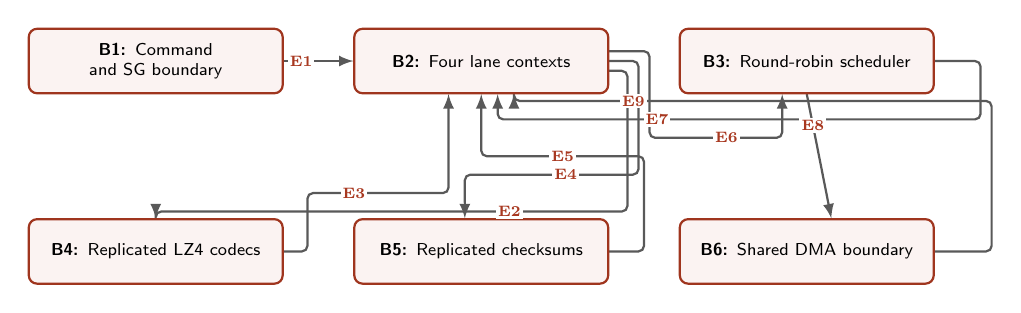
\begin{tikzpicture}[scale=0.78,transform shape,every node/.style={font=\footnotesize\sffamily},>=latex]

\node[draw=vulcan!85!black,thick,rounded corners=3pt,fill=vulcan!6,text width=3.9cm,minimum height=1.05cm,align=center] (b0) at (0.0,0.0) {\textbf{B1:} Comm\allowbreak{}and and SG boun\allowbreak{}dary};

\node[draw=vulcan!85!black,thick,rounded corners=3pt,fill=vulcan!6,text width=3.9cm,minimum height=1.05cm,align=center] (b1) at (5.3,0.0) {\textbf{B2:} Four lane cont\allowbreak{}exts};

\node[draw=vulcan!85!black,thick,rounded corners=3pt,fill=vulcan!6,text width=3.9cm,minimum height=1.05cm,align=center] (b2) at (10.6,0.0) {\textbf{B3:} Roun\allowbreak{}d-robi\allowbreak{}n sche\allowbreak{}dule\allowbreak{}r};

\node[draw=vulcan!85!black,thick,rounded corners=3pt,fill=vulcan!6,text width=3.9cm,minimum height=1.05cm,align=center] (b3) at (0.0,-3.1) {\textbf{B4:} Repl\allowbreak{}icat\allowbreak{}ed LZ4 code\allowbreak{}cs};

\node[draw=vulcan!85!black,thick,rounded corners=3pt,fill=vulcan!6,text width=3.9cm,minimum height=1.05cm,align=center] (b4) at (5.3,-3.1) {\textbf{B5:} Repl\allowbreak{}icat\allowbreak{}ed chec\allowbreak{}ksum\allowbreak{}s};

\node[draw=vulcan!85!black,thick,rounded corners=3pt,fill=vulcan!6,text width=3.9cm,minimum height=1.05cm,align=center] (b5) at (10.6,-3.1) {\textbf{B6:} Shar\allowbreak{}ed DMA boun\allowbreak{}dary};

\begin{pgfonlayer}{connections}

\draw[->,thick,black!65] ([yshift=0.000cm]b0.east) -- coordinate[pos=0.25] (e0) ([yshift=0.000cm]b1.west);

\draw[->,thick,black!65,rounded corners=2pt] ([yshift=-0.160cm]b1.east) -- (7.680,-0.160) -- (7.680,-2.450) -- coordinate[pos=0.25] (e1) (0.000,-2.450) -- ([xshift=0.000cm]b3.north);

\draw[->,thick,black!65,rounded corners=2pt] ([yshift=0.000cm]b3.east) -- (2.470,-3.100) -- (2.470,-2.150) -- coordinate[pos=0.33] (e2) (4.767,-2.150) -- ([xshift=-0.533cm]b1.south);

\draw[->,thick,black!65,rounded corners=2pt] ([yshift=0.000cm]b1.east) -- (7.860,0.000) -- (7.860,-1.850) -- coordinate[pos=0.42] (e3) (5.033,-1.850) -- ([xshift=-0.267cm]b4.north);

\draw[->,thick,black!65,rounded corners=2pt] ([yshift=0.000cm]b4.east) -- (7.950,-3.100) -- (7.950,-1.550) -- coordinate[pos=0.50] (e4) (5.300,-1.550) -- ([xshift=0.000cm]b1.south);

\draw[->,thick,black!65,rounded corners=2pt] ([yshift=0.160cm]b1.east) -- (8.040,0.160) -- (8.040,-1.250) -- coordinate[pos=0.58] (e5) (10.200,-1.250) -- ([xshift=-0.400cm]b2.south);

\draw[->,thick,black!65,rounded corners=2pt] ([yshift=0.000cm]b2.east) -- (13.430,0.000) -- (13.430,-0.950) -- coordinate[pos=0.67] (e6) (5.567,-0.950) -- ([xshift=0.267cm]b1.south);

\draw[->,thick,black!65] ([xshift=0.000cm]b2.south) -- coordinate[pos=0.25] (e7) ([xshift=0.400cm]b5.north);

\draw[->,thick,black!65,rounded corners=2pt] ([yshift=0.000cm]b5.east) -- (13.610,-3.100) -- (13.610,-0.650) -- coordinate[pos=0.75] (e8) (5.833,-0.650) -- ([xshift=0.533cm]b1.south);

\end{pgfonlayer}

\begin{pgfonlayer}{edge labels}

\node[fill=white,inner sep=1pt,font=\scriptsize\bfseries,text=vulcan!90!black] at (e0) {E1};

\node[fill=white,inner sep=1pt,font=\scriptsize\bfseries,text=vulcan!90!black] at (e1) {E2};

\node[fill=white,inner sep=1pt,font=\scriptsize\bfseries,text=vulcan!90!black] at (e2) {E3};

\node[fill=white,inner sep=1pt,font=\scriptsize\bfseries,text=vulcan!90!black] at (e3) {E4};

\node[fill=white,inner sep=1pt,font=\scriptsize\bfseries,text=vulcan!90!black] at (e4) {E5};

\node[fill=white,inner sep=1pt,font=\scriptsize\bfseries,text=vulcan!90!black] at (e5) {E6};

\node[fill=white,inner sep=1pt,font=\scriptsize\bfseries,text=vulcan!90!black] at (e6) {E7};

\node[fill=white,inner sep=1pt,font=\scriptsize\bfseries,text=vulcan!90!black] at (e7) {E8};

\node[fill=white,inner sep=1pt,font=\scriptsize\bfseries,text=vulcan!90!black] at (e8) {E9};

\end{pgfonlayer}

\end{tikzpicture}\par\vspace{3pt}

{\small\textbf{Figure 1:} Top-level microarchitectural functional block map and directed inter-module bus topology.}\end{minipage}\end{center}

{\small\renewcommand{\arraystretch}{1.18}\begin{longtable}{@{}L{0.24\textwidth}|L{0.7\textwidth}@{}}\toprule

\textbf{Bloc\allowbreak{}k} & \textbf{Resp\allowbreak{}onsi\allowbreak{}bili\allowbreak{}ty}\\\midrule\endhead

B1: Comm\allowbreak{}and and SG boun\allowbreak{}dary & Rout\allowbreak{}es comm\allowbreak{}and and desc\allowbreak{}ript\allowbreak{}or hand\allowbreak{}shak\allowbreak{}es to the sele\allowbreak{}cted chan\allowbreak{}nel and expo\allowbreak{}ses lane-spec\allowbreak{}ific avai\allowbreak{}labi\allowbreak{}lity.\\[2pt]\hline

B2: Four lane cont\allowbreak{}exts & lane\allowbreak{}s[\allowbreak{}0..3]\allowbreak{}.cont\allowbreak{}ext reta\allowbreak{}in inde\allowbreak{}pend\allowbreak{}ent comm\allowbreak{}and fiel\allowbreak{}ds,\allowbreak{} SG list\allowbreak{}s,\allowbreak{} coun\allowbreak{}ters,\allowbreak{} inpu\allowbreak{}t/\allowbreak{}outp\allowbreak{}ut slot\allowbreak{}s and fram\allowbreak{}e-cont\allowbreak{}rol stat\allowbreak{}e.\\[2pt]\hline

B3: Roun\allowbreak{}d-robi\allowbreak{}n sche\allowbreak{}dule\allowbreak{}r & sche\allowbreak{}dule\allowbreak{}r cont\allowbreak{}ains inde\allowbreak{}pend\allowbreak{}ent regi\allowbreak{}ster\allowbreak{}ed read,\allowbreak{} writ\allowbreak{}e and comp\allowbreak{}leti\allowbreak{}on arbi\allowbreak{}ters. Pres\allowbreak{}ente\allowbreak{}d sele\allowbreak{}ctio\allowbreak{}ns rema\allowbreak{}in lock\allowbreak{}ed thro\allowbreak{}ugh stal\allowbreak{}ls.\\[2pt]\hline

B4: Repl\allowbreak{}icat\allowbreak{}ed LZ4 code\allowbreak{}cs & Each cont\allowbreak{}ext cont\allowbreak{}ains code\allowbreak{}c:bell\allowbreak{}ows\_\allowbreak{}l2\_\allowbreak{}top,\allowbreak{} reta\allowbreak{}inin\allowbreak{}g comp\allowbreak{}ress\allowbreak{}or matc\allowbreak{}hing/\allowbreak{}emis\allowbreak{}sion and deco\allowbreak{}der hist\allowbreak{}ory/\allowbreak{}outp\allowbreak{}ut hier\allowbreak{}arch\allowbreak{}y.\\[2pt]\hline

B5: Repl\allowbreak{}icat\allowbreak{}ed chec\allowbreak{}ksum\allowbreak{}s & Each cont\allowbreak{}ext cont\allowbreak{}ains chec\allowbreak{}ksum:bell\allowbreak{}ows\_\allowbreak{}l3\_\allowbreak{}chec\allowbreak{}ksum,\allowbreak{} usin\allowbreak{}g sequ\allowbreak{}enti\allowbreak{}al CRC step\allowbreak{}s and regi\allowbreak{}ster\allowbreak{}ed XXH3\allowbreak{}2 arit\allowbreak{}hmet\allowbreak{}ic.\\[2pt]\hline

B6: Shar\allowbreak{}ed DMA boun\allowbreak{}dary & dma:bell\allowbreak{}ows\_\allowbreak{}l3\_\allowbreak{}sg\_\allowbreak{}dma trac\allowbreak{}ks one outs\allowbreak{}tand\allowbreak{}ing read and one outs\allowbreak{}tand\allowbreak{}ing writ\allowbreak{}e inde\allowbreak{}pend\allowbreak{}entl\allowbreak{}y and rout\allowbreak{}es orde\allowbreak{}red resp\allowbreak{}onse\allowbreak{}s to capt\allowbreak{}ured owne\allowbreak{}rs.\\[2pt]\hline

\bottomrule\end{longtable}}

{\small\renewcommand{\arraystretch}{1.18}\begin{longtable}{@{}L{0.24\textwidth}|L{0.7\textwidth}@{}}\toprule

\textbf{Dire\allowbreak{}cted rela\allowbreak{}tion\allowbreak{}ship} & \textbf{Mean\allowbreak{}ing}\\\midrule\endhead

E1: B1 to B2 & Acce\allowbreak{}pted comm\allowbreak{}ands and desc\allowbreak{}ript\allowbreak{}ors\\[2pt]\hline

E2: B2 to B4 & Payl\allowbreak{}oad inpu\allowbreak{}t and code\allowbreak{}c cont\allowbreak{}rol\\[2pt]\hline

E3: B4 to B2 & Enco\allowbreak{}ded/\allowbreak{}deco\allowbreak{}ded byte\allowbreak{}s and code\allowbreak{}c stat\allowbreak{}us\\[2pt]\hline

E4: B2 to B5 & Acce\allowbreak{}pted cont\allowbreak{}ent byte\allowbreak{}s and fina\allowbreak{}liza\allowbreak{}tion\\[2pt]\hline

E5: B5 to B2 & Comp\allowbreak{}uted cont\allowbreak{}ent chec\allowbreak{}ksum\\[2pt]\hline

E6: B2 to B3 & Elig\allowbreak{}ible requ\allowbreak{}ests and comp\allowbreak{}leti\allowbreak{}on payl\allowbreak{}oads\\[2pt]\hline

E7: B3 to B2 & Rese\allowbreak{}rvat\allowbreak{}ions and comp\allowbreak{}leti\allowbreak{}on reti\allowbreak{}reme\allowbreak{}nt\\[2pt]\hline

E8: B3 to B6 & Regi\allowbreak{}ster\allowbreak{}ed requ\allowbreak{}ests with chan\allowbreak{}nel owne\allowbreak{}rshi\allowbreak{}p\\[2pt]\hline

E9: B6 to B2 & Read resp\allowbreak{}onse\allowbreak{}s and writ\allowbreak{}e ackn\allowbreak{}owle\allowbreak{}dgme\allowbreak{}nts\\[2pt]\hline

\bottomrule\end{longtable}}

\needspace{9\baselineskip}\section{Interfaces and configuration}

{\small\renewcommand{\arraystretch}{1.18}\begin{longtable}{@{}L{0.21\textwidth}|L{0.12\textwidth}|L{0.12\textwidth}|L{0.45\textwidth}@{}}\toprule

\textbf{Sign\allowbreak{}al /\allowbreak{} grou\allowbreak{}p} & \textbf{Dire\allowbreak{}ctio\allowbreak{}n} & \textbf{Widt\allowbreak{}h} & \textbf{Cont\allowbreak{}ract}\\\midrule\endhead

clk,\allowbreak{} rst\_\allowbreak{}n & Inpu\allowbreak{}t & 1 bit each & Sing\allowbreak{}le risi\allowbreak{}ng-edge cloc\allowbreak{}k and asyn\allowbreak{}chro\allowbreak{}nous acti\allowbreak{}ve-low cont\allowbreak{}rol rese\allowbreak{}t. Ever\allowbreak{}y publ\allowbreak{}ic outp\allowbreak{}ut is zero duri\allowbreak{}ng rese\allowbreak{}t. The exte\allowbreak{}rnal brid\allowbreak{}ge must disc\allowbreak{}ard pre-rese\allowbreak{}t tran\allowbreak{}sact\allowbreak{}ions.\\[2pt]\hline

Comm\allowbreak{}and & Inpu\allowbreak{}t payl\allowbreak{}oad/\allowbreak{}vali\allowbreak{}d; outp\allowbreak{}ut read\allowbreak{}y & cmd\_\allowbreak{}vali\allowbreak{}d,\allowbreak{} cmd\_\allowbreak{}read\allowbreak{}y,\allowbreak{} cmd\_\allowbreak{}deco\allowbreak{}mpre\allowbreak{}ss: 1; cmd\_\allowbreak{}chan\allowbreak{}nel,\allowbreak{} cmd\_\allowbreak{}chec\allowbreak{}ksum\_\allowbreak{}mode: 2; cmd\_\allowbreak{}id: 16; cmd\_\allowbreak{}src\_\allowbreak{}byte\allowbreak{}s,\allowbreak{} cmd\_\allowbreak{}dst\_\allowbreak{}capa\allowbreak{}city: 32; cmd\_\allowbreak{}src\_\allowbreak{}segm\allowbreak{}ents,\allowbreak{} cmd\_\allowbreak{}dst\_\allowbreak{}segm\allowbreak{}ents: 5 & Fiel\allowbreak{}ds snap\allowbreak{}shot only on cmd\_\allowbreak{}vali\allowbreak{}d \&\& cmd\_\allowbreak{}read\allowbreak{}y. Dire\allowbreak{}ctio\allowbreak{}n 0 comp\allowbreak{}ress\allowbreak{}es; 1 deco\allowbreak{}mpre\allowbreak{}sses. Chec\allowbreak{}ksum mode\allowbreak{}s are 0 none,\allowbreak{} 1 XXH3\allowbreak{}2,\allowbreak{} 2 CRC3\allowbreak{}2; 3 is inva\allowbreak{}lid. A chan\allowbreak{}nel rema\allowbreak{}ins busy unti\allowbreak{}l its comp\allowbreak{}leti\allowbreak{}on tran\allowbreak{}sfer\allowbreak{}s.\\[2pt]\hline

Scat\allowbreak{}ter-gath\allowbreak{}er desc\allowbreak{}ript\allowbreak{}ors & Inpu\allowbreak{}t payl\allowbreak{}oad/\allowbreak{}vali\allowbreak{}d; outp\allowbreak{}ut read\allowbreak{}y & sg\_\allowbreak{}vali\allowbreak{}d,\allowbreak{} sg\_\allowbreak{}read\allowbreak{}y,\allowbreak{} sg\_\allowbreak{}dest\allowbreak{}inat\allowbreak{}ion: 1; sg\_\allowbreak{}chan\allowbreak{}nel: 2; sg\_\allowbreak{}addr: 64; sg\_\allowbreak{}byte\allowbreak{}s: 32 & sg\_\allowbreak{}dest\allowbreak{}inat\allowbreak{}ion sele\allowbreak{}cts sour\allowbreak{}ce=\allowbreak{}0 or dest\allowbreak{}inat\allowbreak{}ion=\allowbreak{}1. Acce\allowbreak{}ptan\allowbreak{}ce orde\allowbreak{}r defi\allowbreak{}nes conc\allowbreak{}aten\allowbreak{}atio\allowbreak{}n with\allowbreak{}in each chan\allowbreak{}nel/\allowbreak{}dire\allowbreak{}ctio\allowbreak{}n. All decl\allowbreak{}ared desc\allowbreak{}ript\allowbreak{}ors must arri\allowbreak{}ve and vali\allowbreak{}date befo\allowbreak{}re DMA begi\allowbreak{}ns.\\[2pt]\hline

DMA read & Outp\allowbreak{}ut requ\allowbreak{}est/\allowbreak{}inpu\allowbreak{}t read\allowbreak{}y; inpu\allowbreak{}t resp\allowbreak{}onse/\allowbreak{}outp\allowbreak{}ut read\allowbreak{}y & rd\_\allowbreak{}req\_\allowbreak{}vali\allowbreak{}d,\allowbreak{} rd\_\allowbreak{}req\_\allowbreak{}read\allowbreak{}y,\allowbreak{} rd\_\allowbreak{}rsp\_\allowbreak{}vali\allowbreak{}d,\allowbreak{} rd\_\allowbreak{}rsp\_\allowbreak{}read\allowbreak{}y,\allowbreak{} rd\_\allowbreak{}rsp\_\allowbreak{}erro\allowbreak{}r: 1; rd\_\allowbreak{}req\_\allowbreak{}chan\allowbreak{}nel: 2; rd\_\allowbreak{}req\_\allowbreak{}addr: 64; rd\_\allowbreak{}rsp\_\allowbreak{}data: 8 & Each acce\allowbreak{}pted requ\allowbreak{}est read\allowbreak{}s one byte. At most one read is glob\allowbreak{}ally outs\allowbreak{}tand\allowbreak{}ing. Resp\allowbreak{}onse\allowbreak{}s are orde\allowbreak{}red and unta\allowbreak{}gged,\allowbreak{} exac\allowbreak{}tly one per acce\allowbreak{}pted requ\allowbreak{}est,\allowbreak{} no earl\allowbreak{}ier than the foll\allowbreak{}owin\allowbreak{}g edge.\\[2pt]\hline

DMA writ\allowbreak{}e & Outp\allowbreak{}ut requ\allowbreak{}est/\allowbreak{}inpu\allowbreak{}t read\allowbreak{}y; inpu\allowbreak{}t ackn\allowbreak{}owle\allowbreak{}dgme\allowbreak{}nt/\allowbreak{}outp\allowbreak{}ut read\allowbreak{}y & wr\_\allowbreak{}req\_\allowbreak{}vali\allowbreak{}d,\allowbreak{} wr\_\allowbreak{}req\_\allowbreak{}read\allowbreak{}y,\allowbreak{} wr\_\allowbreak{}rsp\_\allowbreak{}vali\allowbreak{}d,\allowbreak{} wr\_\allowbreak{}rsp\_\allowbreak{}read\allowbreak{}y,\allowbreak{} wr\_\allowbreak{}rsp\_\allowbreak{}erro\allowbreak{}r: 1; wr\_\allowbreak{}req\_\allowbreak{}chan\allowbreak{}nel: 2; wr\_\allowbreak{}req\_\allowbreak{}addr: 64; wr\_\allowbreak{}req\_\allowbreak{}data: 8 & Each acce\allowbreak{}pted requ\allowbreak{}est writ\allowbreak{}es one byte. At most one writ\allowbreak{}e is glob\allowbreak{}ally outs\allowbreak{}tand\allowbreak{}ing,\allowbreak{} inde\allowbreak{}pend\allowbreak{}entl\allowbreak{}y of read\allowbreak{}s. Comp\allowbreak{}leti\allowbreak{}on acco\allowbreak{}unti\allowbreak{}ng adva\allowbreak{}nces on succ\allowbreak{}essf\allowbreak{}ul ackn\allowbreak{}owle\allowbreak{}dgme\allowbreak{}nts,\allowbreak{} not requ\allowbreak{}est pres\allowbreak{}enta\allowbreak{}tion.\\[2pt]\hline

Comp\allowbreak{}leti\allowbreak{}on & Outp\allowbreak{}ut payl\allowbreak{}oad/\allowbreak{}vali\allowbreak{}d; inpu\allowbreak{}t read\allowbreak{}y & stat\allowbreak{}us\_\allowbreak{}vali\allowbreak{}d,\allowbreak{} stat\allowbreak{}us\_\allowbreak{}read\allowbreak{}y,\allowbreak{} err\_\allowbreak{}chec\allowbreak{}ksum\_\allowbreak{}mism\allowbreak{}atch: 1; stat\allowbreak{}us\_\allowbreak{}chan\allowbreak{}nel: 2; stat\allowbreak{}us\_\allowbreak{}id: 16; stat\allowbreak{}us\_\allowbreak{}erro\allowbreak{}r: 4; stat\allowbreak{}us\_\allowbreak{}src\_\allowbreak{}byte\allowbreak{}s,\allowbreak{} stat\allowbreak{}us\_\allowbreak{}dst\_\allowbreak{}byte\allowbreak{}s,\allowbreak{} stat\allowbreak{}us\_\allowbreak{}chec\allowbreak{}ksum: 32 & Exac\allowbreak{}tly one comp\allowbreak{}leti\allowbreak{}on is prod\allowbreak{}uced per non-rese\allowbreak{}t-abor\allowbreak{}ted comm\allowbreak{}and. Coun\allowbreak{}ts repo\allowbreak{}rt cons\allowbreak{}umed read resp\allowbreak{}onse\allowbreak{}s and succ\allowbreak{}essf\allowbreak{}ul writ\allowbreak{}e ackn\allowbreak{}owle\allowbreak{}dgme\allowbreak{}nts. err\_\allowbreak{}chec\allowbreak{}ksum\_\allowbreak{}mism\allowbreak{}atch equa\allowbreak{}ls stat\allowbreak{}us\_\allowbreak{}vali\allowbreak{}d \&\& stat\allowbreak{}us\_\allowbreak{}erro\allowbreak{}r=\allowbreak{}=\allowbreak{}7. Vali\allowbreak{}d payl\allowbreak{}oads rema\allowbreak{}in stab\allowbreak{}le thro\allowbreak{}ugh stal\allowbreak{}ls. All inte\allowbreak{}rfac\allowbreak{}e fiel\allowbreak{}ds are unsi\allowbreak{}gned [\allowbreak{}E002,\allowbreak{} E015]\allowbreak{}.\\[2pt]\hline

\bottomrule\end{longtable}}

{\small\renewcommand{\arraystretch}{1.18}\begin{longtable}{@{}L{0.22\textwidth}|L{0.21\textwidth}|L{0.49\textwidth}@{}}\toprule

\textbf{Para\allowbreak{}mete\allowbreak{}r} & \textbf{Defa\allowbreak{}ult} & \textbf{Mean\allowbreak{}ing /\allowbreak{} supp\allowbreak{}orte\allowbreak{}d valu\allowbreak{}es}\\\midrule\endhead

MAX\_\allowbreak{}BLOC\allowbreak{}K\_\allowbreak{}BYTE\allowbreak{}S & 6553\allowbreak{}6 & Inte\allowbreak{}ger 1..6553\allowbreak{}6 incl\allowbreak{}usiv\allowbreak{}e; boun\allowbreak{}ds comp\allowbreak{}ress\allowbreak{}ion inpu\allowbreak{}t and succ\allowbreak{}essf\allowbreak{}ul L3 deco\allowbreak{}ded cont\allowbreak{}ent. Stan\allowbreak{}dalo\allowbreak{}ne pare\allowbreak{}nt deco\allowbreak{}ding reta\allowbreak{}ins unbo\allowbreak{}unde\allowbreak{}d-outp\allowbreak{}ut beha\allowbreak{}vior.\\[2pt]\hline

SG\_\allowbreak{}DEPT\allowbreak{}H & 16 & Inte\allowbreak{}ger 1..16 incl\allowbreak{}usiv\allowbreak{}e,\allowbreak{} incl\allowbreak{}udin\allowbreak{}g non-powe\allowbreak{}rs of two. Boun\allowbreak{}ds each sour\allowbreak{}ce/\allowbreak{}dest\allowbreak{}inat\allowbreak{}ion desc\allowbreak{}ript\allowbreak{}or list per lane. Four chan\allowbreak{}nels are fixe\allowbreak{}d,\allowbreak{} not para\allowbreak{}mete\allowbreak{}rize\allowbreak{}d. Ille\allowbreak{}gal para\allowbreak{}mete\allowbreak{}r valu\allowbreak{}es use diag\allowbreak{}nost\allowbreak{}ic-safe stor\allowbreak{}age and issu\allowbreak{}e PARA\allowbreak{}METE\allowbreak{}R ERRO\allowbreak{}R at simu\allowbreak{}lati\allowbreak{}on star\allowbreak{}tup [\allowbreak{}E015,\allowbreak{} E167]\allowbreak{}.\\[2pt]\hline

\bottomrule\end{longtable}}

\needspace{16\baselineskip}\section{Behavior and corner cases}

\subsection{Desc\allowbreak{}ript\allowbreak{}or vali\allowbreak{}dati\allowbreak{}on}

Segm\allowbreak{}ents requ\allowbreak{}ire posi\allowbreak{}tive leng\allowbreak{}ths and nono\allowbreak{}verf\allowbreak{}lowi\allowbreak{}ng incl\allowbreak{}usiv\allowbreak{}e 64-bit addr\allowbreak{}ess rang\allowbreak{}es. Wide\allowbreak{}ned sour\allowbreak{}ce and dest\allowbreak{}inat\allowbreak{}ion sums must exac\allowbreak{}tly equa\allowbreak{}l comm\allowbreak{}and leng\allowbreak{}ths. Dest\allowbreak{}inat\allowbreak{}ion capa\allowbreak{}city/\allowbreak{}coun\allowbreak{}t are nonz\allowbreak{}ero; sour\allowbreak{}ce coun\allowbreak{}t is zero exac\allowbreak{}tly for zero-leng\allowbreak{}th comp\allowbreak{}ress\allowbreak{}ion. Coun\allowbreak{}ts cann\allowbreak{}ot exce\allowbreak{}ed SG\_\allowbreak{}DEPT\allowbreak{}H. Comp\allowbreak{}ress\allowbreak{}ion sour\allowbreak{}ce leng\allowbreak{}th is at most MAX\_\allowbreak{}BLOC\allowbreak{}K\_\allowbreak{}BYTE\allowbreak{}S. Deco\allowbreak{}mpre\allowbreak{}ssio\allowbreak{}n sour\allowbreak{}ce leng\allowbreak{}th rang\allowbreak{}es from one payl\allowbreak{}oad byte plus trai\allowbreak{}ler thro\allowbreak{}ugh 2*\allowbreak{}MAX\_\allowbreak{}BLOC\allowbreak{}K\_\allowbreak{}BYTE\allowbreak{}S+\allowbreak{}20. Inva\allowbreak{}lid comm\allowbreak{}ands acce\allowbreak{}pt no desc\allowbreak{}ript\allowbreak{}ors; inva\allowbreak{}lid list\allowbreak{}s cons\allowbreak{}ume rema\allowbreak{}inin\allowbreak{}g decl\allowbreak{}ared desc\allowbreak{}ript\allowbreak{}ors befo\allowbreak{}re comp\allowbreak{}leti\allowbreak{}ng with\allowbreak{}out DMA. Unal\allowbreak{}igne\allowbreak{}d segm\allowbreak{}ents are supp\allowbreak{}orte\allowbreak{}d; boun\allowbreak{}dari\allowbreak{}es inse\allowbreak{}rt no byte\allowbreak{}s or code\allowbreak{}c rese\allowbreak{}ts.

\needspace{10\baselineskip}\subsection{Fram\allowbreak{}ing and comp\allowbreak{}atib\allowbreak{}ilit\allowbreak{}y}

A fram\allowbreak{}e is one inde\allowbreak{}pend\allowbreak{}ent raw LZ4 bloc\allowbreak{}k foll\allowbreak{}owed,\allowbreak{} when enab\allowbreak{}led,\allowbreak{} by four litt\allowbreak{}le-endi\allowbreak{}an chec\allowbreak{}ksum byte\allowbreak{}s. It is not the stan\allowbreak{}dard LZ4 Fram\allowbreak{}e head\allowbreak{}er form\allowbreak{}at. Empt\allowbreak{}y comp\allowbreak{}ress\allowbreak{}ion emit\allowbreak{}s toke\allowbreak{}n 00 and its opti\allowbreak{}onal trai\allowbreak{}ler; empt\allowbreak{}y deco\allowbreak{}ding prod\allowbreak{}uces no writ\allowbreak{}es. No dict\allowbreak{}iona\allowbreak{}ry surv\allowbreak{}ives a fram\allowbreak{}e. Comp\allowbreak{}ress\allowbreak{}ion reta\allowbreak{}ins genu\allowbreak{}ine matc\allowbreak{}hes. Pare\allowbreak{}nt stan\allowbreak{}dalo\allowbreak{}ne roun\allowbreak{}dtri\allowbreak{}p\_\allowbreak{}enab\allowbreak{}le,\allowbreak{} keep hand\allowbreak{}ling,\allowbreak{} over\allowbreak{}lap copi\allowbreak{}es,\allowbreak{} exte\allowbreak{}nsio\allowbreak{}ns and hist\allowbreak{}ory-wrap beha\allowbreak{}vior rema\allowbreak{}in avai\allowbreak{}labl\allowbreak{}e; L3 ties roun\allowbreak{}dtri\allowbreak{}p\_\allowbreak{}enab\allowbreak{}le low [\allowbreak{}E001–E010]\allowbreak{}.

\needspace{10\baselineskip}\subsection{Exac\allowbreak{}t chec\allowbreak{}ksum arit\allowbreak{}hmet\allowbreak{}ic}

Chec\allowbreak{}ksum\allowbreak{}s cove\allowbreak{}r unco\allowbreak{}mpre\allowbreak{}ssed cont\allowbreak{}ent once per acce\allowbreak{}pted logi\allowbreak{}cal byte. XXH3\allowbreak{}2 uses seed zero,\allowbreak{} litt\allowbreak{}le-endi\allowbreak{}an word\allowbreak{}s,\allowbreak{} modu\allowbreak{}lo-2\textasciicircum{}32 arit\allowbreak{}hmet\allowbreak{}ic,\allowbreak{} logi\allowbreak{}cal shif\allowbreak{}ts and hexa\allowbreak{}deci\allowbreak{}mal prim\allowbreak{}es P1=\allowbreak{}9E37\allowbreak{}79B1,\allowbreak{} P2=\allowbreak{}85EB\allowbreak{}CA77,\allowbreak{} P3=\allowbreak{}C2B2\allowbreak{}AE3D,\allowbreak{} P4=\allowbreak{}27D4\allowbreak{}EB2F,\allowbreak{} P5=\allowbreak{}1656\allowbreak{}67B1. Stri\allowbreak{}pe lane\allowbreak{}s star\allowbreak{}t at P1+\allowbreak{}P2,\allowbreak{} P2,\allowbreak{} 0,\allowbreak{} -P1 and upda\allowbreak{}te as rotl(\allowbreak{}v+\allowbreak{}word*\allowbreak{}P2,\allowbreak{}13)\allowbreak{}*\allowbreak{}P1. Rota\allowbreak{}tion\allowbreak{}s 1,\allowbreak{}7,\allowbreak{}12,\allowbreak{}18 comb\allowbreak{}ine lane\allowbreak{}s with\allowbreak{}out an XXH6\allowbreak{}4 merg\allowbreak{}e roun\allowbreak{}d; shor\allowbreak{}t inpu\allowbreak{}ts star\allowbreak{}t at P5. Afte\allowbreak{}r addi\allowbreak{}ng leng\allowbreak{}th,\allowbreak{} tail word\allowbreak{}s use rotl(\allowbreak{}h+\allowbreak{}word*\allowbreak{}P3,\allowbreak{}17)\allowbreak{}*\allowbreak{}P4 and byte\allowbreak{}s use rotl(\allowbreak{}h+\allowbreak{}byte*\allowbreak{}P5,\allowbreak{}11)\allowbreak{}*\allowbreak{}P1. Aval\allowbreak{}anch\allowbreak{}e appl\allowbreak{}ies xor-shif\allowbreak{}t15,\allowbreak{} mult\allowbreak{}iply P2,\allowbreak{} xor-shif\allowbreak{}t13,\allowbreak{} mult\allowbreak{}iply P3,\allowbreak{} xor-shif\allowbreak{}t16. CRC-32/\allowbreak{}ISO-HDLC init\allowbreak{}iali\allowbreak{}zes FFFF\allowbreak{}FFFF,\allowbreak{} uses refl\allowbreak{}ecte\allowbreak{}d poly\allowbreak{}nomi\allowbreak{}al EDB8\allowbreak{}8320 and fina\allowbreak{}l XOR FFFF\allowbreak{}FFFF. Know\allowbreak{}n answ\allowbreak{}ers are XXH3\allowbreak{}2(\allowbreak{}empt\allowbreak{}y)\allowbreak{}=\allowbreak{}02CC\allowbreak{}5D05,\allowbreak{} XXH3\allowbreak{}2(\allowbreak{}abc)\allowbreak{}=\allowbreak{}32D1\allowbreak{}53FF and CRC3\allowbreak{}2(\allowbreak{}1234\allowbreak{}5678\allowbreak{}9)\allowbreak{}=\allowbreak{}CBF4\allowbreak{}3926. Mode none repo\allowbreak{}rts zero [\allowbreak{}E002,\allowbreak{} E011,\allowbreak{} E018]\allowbreak{}.

\needspace{10\baselineskip}\subsection{Regi\allowbreak{}ster\allowbreak{}ed sche\allowbreak{}duli\allowbreak{}ng}

Comm\allowbreak{}ands acce\allowbreak{}pted at E0 firs\allowbreak{}t perm\allowbreak{}it desc\allowbreak{}ript\allowbreak{}ors at E1. A fina\allowbreak{}l desc\allowbreak{}ript\allowbreak{}or at Ek ente\allowbreak{}rs VALI\allowbreak{}DATE; Ek+\allowbreak{}1 ente\allowbreak{}rs ARM,\allowbreak{} Ek+\allowbreak{}2 ente\allowbreak{}rs RUN,\allowbreak{} and the shar\allowbreak{}ed requ\allowbreak{}est slot can load at Ek+\allowbreak{}3. Read resp\allowbreak{}onse\allowbreak{}s ente\allowbreak{}r a lane hold\allowbreak{}ing regi\allowbreak{}ster befo\allowbreak{}re code\allowbreak{}c tran\allowbreak{}sfer. Code\allowbreak{}c outp\allowbreak{}ut capt\allowbreak{}ured at Ec can load the shar\allowbreak{}ed writ\allowbreak{}e regi\allowbreak{}ster at Ec+\allowbreak{}1 and firs\allowbreak{}t tran\allowbreak{}sfer at Ec+\allowbreak{}2. Comp\allowbreak{}leti\allowbreak{}on uses sett\allowbreak{}leme\allowbreak{}nt and shar\allowbreak{}ed-stat\allowbreak{}us regi\allowbreak{}ster\allowbreak{}s afte\allowbreak{}r fina\allowbreak{}l ackn\allowbreak{}owle\allowbreak{}dgme\allowbreak{}nt/\allowbreak{}inte\allowbreak{}rnal fini\allowbreak{}sh. Cont\allowbreak{}inuo\allowbreak{}usly elig\allowbreak{}ible lane\allowbreak{}s rece\allowbreak{}ive serv\allowbreak{}ice with\allowbreak{}in four acce\allowbreak{}pted gran\allowbreak{}ts; exte\allowbreak{}rnal stal\allowbreak{}ls exte\allowbreak{}nd late\allowbreak{}ncy.

\needspace{10\baselineskip}\subsection{Chec\allowbreak{}ksum exec\allowbreak{}utio\allowbreak{}n late\allowbreak{}ncy}

CRC perf\allowbreak{}orms eigh\allowbreak{}t bit-upda\allowbreak{}te edge\allowbreak{}s per byte; succ\allowbreak{}essi\allowbreak{}ve byte acce\allowbreak{}ptan\allowbreak{}ce is at leas\allowbreak{}t nine edge\allowbreak{}s apar\allowbreak{}t. XXH3\allowbreak{}2 proc\allowbreak{}esse\allowbreak{}s each comp\allowbreak{}lete stri\allowbreak{}pe in 20 arit\allowbreak{}hmet\allowbreak{}ic/\allowbreak{}stor\allowbreak{}age edge\allowbreak{}s,\allowbreak{} acce\allowbreak{}ptin\allowbreak{}g the next byte no earl\allowbreak{}ier than edge 21 afte\allowbreak{}r stri\allowbreak{}pe-comp\allowbreak{}leti\allowbreak{}ng acce\allowbreak{}ptan\allowbreak{}ce. Afte\allowbreak{}r acce\allowbreak{}pted fini\allowbreak{}sh F,\allowbreak{} XXH3\allowbreak{}2 prod\allowbreak{}uces its resu\allowbreak{}lt at F+\allowbreak{}7+\allowbreak{}6W+\allowbreak{}6B for shor\allowbreak{}t inpu\allowbreak{}ts or F+\allowbreak{}10+\allowbreak{}6W+\allowbreak{}6B afte\allowbreak{}r stri\allowbreak{}pes,\allowbreak{} wher\allowbreak{}e W and B are rema\allowbreak{}inin\allowbreak{}g word\allowbreak{}s and byte\allowbreak{}s. Thes\allowbreak{}e loca\allowbreak{}l sche\allowbreak{}dule\allowbreak{}s do not esta\allowbreak{}blis\allowbreak{}h fixe\allowbreak{}d fram\allowbreak{}e late\allowbreak{}ncy [\allowbreak{}E001]\allowbreak{}.

\needspace{10\baselineskip}\subsection{Erro\allowbreak{}rs and reco\allowbreak{}very}

Code\allowbreak{}s are 0 succ\allowbreak{}ess,\allowbreak{} 1 malf\allowbreak{}orme\allowbreak{}d/\allowbreak{}trun\allowbreak{}cate\allowbreak{}d boun\allowbreak{}dary or miss\allowbreak{}ing trai\allowbreak{}ler,\allowbreak{} 2 zero offs\allowbreak{}et,\allowbreak{} 3 unav\allowbreak{}aila\allowbreak{}ble hist\allowbreak{}ory,\allowbreak{} 4 leng\allowbreak{}th over\allowbreak{}flow,\allowbreak{} 5 bloc\allowbreak{}k limi\allowbreak{}t,\allowbreak{} 6 pare\allowbreak{}nt inva\allowbreak{}lid keep,\allowbreak{} 7 chec\allowbreak{}ksum mism\allowbreak{}atch,\allowbreak{} 8 comm\allowbreak{}and/\allowbreak{}desc\allowbreak{}ript\allowbreak{}or erro\allowbreak{}r,\allowbreak{} 9 capa\allowbreak{}city exha\allowbreak{}usti\allowbreak{}on and 10 DMA erro\allowbreak{}r. The firs\allowbreak{}t dete\allowbreak{}cted proc\allowbreak{}essi\allowbreak{}ng erro\allowbreak{}r is reta\allowbreak{}ined. New lane tran\allowbreak{}sact\allowbreak{}ions stop whil\allowbreak{}e alre\allowbreak{}ady pres\allowbreak{}ente\allowbreak{}d/\allowbreak{}acce\allowbreak{}pted bus work sett\allowbreak{}les. Enab\allowbreak{}led mode\allowbreak{}s repo\allowbreak{}rt the comp\allowbreak{}uted chec\allowbreak{}ksum,\allowbreak{} incl\allowbreak{}udin\allowbreak{}g on mism\allowbreak{}atch. Deco\allowbreak{}ded writ\allowbreak{}es are untr\allowbreak{}uste\allowbreak{}d unti\allowbreak{}l succ\allowbreak{}essf\allowbreak{}ul comp\allowbreak{}leti\allowbreak{}on; no roll\allowbreak{}back is prov\allowbreak{}ided.

\needspace{10\baselineskip}\subsection{Rese\allowbreak{}t and chan\allowbreak{}nel reus\allowbreak{}e}

Rese\allowbreak{}t abor\allowbreak{}ts cont\allowbreak{}exts and clea\allowbreak{}rs pend\allowbreak{}ing requ\allowbreak{}ests,\allowbreak{} owne\allowbreak{}rshi\allowbreak{}p and stat\allowbreak{}us with\allowbreak{}out clea\allowbreak{}ring larg\allowbreak{}e memo\allowbreak{}ries. The brid\allowbreak{}ge must rese\allowbreak{}t/\allowbreak{}drai\allowbreak{}n conc\allowbreak{}urre\allowbreak{}ntly and must not retu\allowbreak{}rn stal\allowbreak{}e resp\allowbreak{}onse\allowbreak{}s. Rese\allowbreak{}t take\allowbreak{}s prec\allowbreak{}eden\allowbreak{}ce over hand\allowbreak{}shak\allowbreak{}es. A chan\allowbreak{}nel rema\allowbreak{}ins busy thro\allowbreak{}ugh comp\allowbreak{}leti\allowbreak{}on reti\allowbreak{}reme\allowbreak{}nt and acce\allowbreak{}pts its next comm\allowbreak{}and on a late\allowbreak{}r edge [\allowbreak{}E002]\allowbreak{}.

\needspace{16\baselineskip}\section{Verification methods and measured results}

\subsection{Soft\allowbreak{}ware-vs-Hard\allowbreak{}ware nume\allowbreak{}rica\allowbreak{}l comp\allowbreak{}aris\allowbreak{}on}

\textbf{Method.} Comp\allowbreak{}iled Veri\allowbreak{}lato\allowbreak{}r RTL agai\allowbreak{}nst inde\allowbreak{}pend\allowbreak{}ent Pyth\allowbreak{}on LZ4 pars\allowbreak{}ing/\allowbreak{}bloc\allowbreak{}k gene\allowbreak{}rati\allowbreak{}on,\allowbreak{} cano\allowbreak{}nica\allowbreak{}l XXH3\allowbreak{}2 and zlib CRC3\allowbreak{}2,\allowbreak{} with publ\allowbreak{}ic DMA byte/\allowbreak{}addr\allowbreak{}ess/\allowbreak{}comp\allowbreak{}leti\allowbreak{}on scor\allowbreak{}eboa\allowbreak{}rds.

\textbf{Result.} 24/\allowbreak{}24 runs pass\allowbreak{}ed: (\allowbreak{}MAX\_\allowbreak{}BLOC\allowbreak{}K\_\allowbreak{}BYTE\allowbreak{}S,\allowbreak{}SG\_\allowbreak{}DEPT\allowbreak{}H)\allowbreak{}=\allowbreak{}(\allowbreak{}1,\allowbreak{}1)\allowbreak{},\allowbreak{}(\allowbreak{}3,\allowbreak{}3)\allowbreak{},\allowbreak{}(\allowbreak{}15,\allowbreak{}1)\allowbreak{},\allowbreak{}(\allowbreak{}16,\allowbreak{}3)\allowbreak{},\allowbreak{}(\allowbreak{}255,\allowbreak{}16)\allowbreak{},\allowbreak{}(\allowbreak{}256,\allowbreak{}3)\allowbreak{},\allowbreak{}(\allowbreak{}4096,\allowbreak{}16)\allowbreak{},\allowbreak{}(\allowbreak{}6553\allowbreak{}6,\allowbreak{}16)\allowbreak{},\allowbreak{} each at seed\allowbreak{}s 17,\allowbreak{}89,\allowbreak{}2027. Each comp\allowbreak{}ared 48 fram\allowbreak{}es acro\allowbreak{}ss all 24 chan\allowbreak{}nel/\allowbreak{}dire\allowbreak{}ctio\allowbreak{}n/\allowbreak{}mode comb\allowbreak{}inat\allowbreak{}ions,\allowbreak{} plus 12 simu\allowbreak{}late\allowbreak{}d DMA roun\allowbreak{}d-trip fram\allowbreak{}es: 1152 matr\allowbreak{}ix fram\allowbreak{}es and 288 addi\allowbreak{}tion\allowbreak{}al roun\allowbreak{}d-trip fram\allowbreak{}es. Per-run resu\allowbreak{}lts are inde\allowbreak{}xed by evid\allowbreak{}ence/\allowbreak{}l1/\allowbreak{}matr\allowbreak{}ix/\allowbreak{}2026\allowbreak{}1029\allowbreak{}T161\allowbreak{}250Z-matr\allowbreak{}ix-eed4\allowbreak{}8dc3/\allowbreak{}matr\allowbreak{}ix-ledg\allowbreak{}er.json.

{\small Evidence: E018,\allowbreak{} E166}

\needspace{12\baselineskip}\subsection{Back\allowbreak{}pres\allowbreak{}sure,\allowbreak{} isol\allowbreak{}atio\allowbreak{}n and erro\allowbreak{}r reco\allowbreak{}very}

\textbf{Method.} Meas\allowbreak{}ured publ\allowbreak{}ic-inte\allowbreak{}rfac\allowbreak{}e cove\allowbreak{}rage,\allowbreak{} dire\allowbreak{}cted malf\allowbreak{}orme\allowbreak{}d/\allowbreak{}desc\allowbreak{}ript\allowbreak{}or/\allowbreak{}DMA/\allowbreak{}capa\allowbreak{}city case\allowbreak{}s,\allowbreak{} rese\allowbreak{}t prob\allowbreak{}es and dedi\allowbreak{}cate\allowbreak{}d sche\allowbreak{}dule\allowbreak{}r/\allowbreak{}erro\allowbreak{}r-sett\allowbreak{}leme\allowbreak{}nt expe\allowbreak{}rime\allowbreak{}nts.

\textbf{Result.} Reco\allowbreak{}rded 2606\allowbreak{}1 chan\allowbreak{}nel swit\allowbreak{}ches,\allowbreak{} four-acti\allowbreak{}ve-cont\allowbreak{}ext cove\allowbreak{}rage,\allowbreak{} at leas\allowbreak{}t 17-cycl\allowbreak{}e read/\allowbreak{}writ\allowbreak{}e/\allowbreak{}stat\allowbreak{}us stal\allowbreak{}ls,\allowbreak{} and 24 occu\allowbreak{}rren\allowbreak{}ces of each rese\allowbreak{}t phas\allowbreak{}e. Sche\allowbreak{}dule\allowbreak{}r test\allowbreak{}ing reco\allowbreak{}rded at leas\allowbreak{}t 64 all-elig\allowbreak{}ible swit\allowbreak{}ches and four-gran\allowbreak{}t fair\allowbreak{}ness. Four erro\allowbreak{}r-sett\allowbreak{}leme\allowbreak{}nt scen\allowbreak{}ario\allowbreak{}s pass\allowbreak{}ed with zero viol\allowbreak{}atio\allowbreak{}ns. The stal\allowbreak{}led-comp\allowbreak{}leti\allowbreak{}on prob\allowbreak{}e was repa\allowbreak{}ired to pres\allowbreak{}erve its read\allowbreak{}ines\allowbreak{}s prec\allowbreak{}ondi\allowbreak{}tion with\allowbreak{}out chan\allowbreak{}ging expe\allowbreak{}cted beha\allowbreak{}vior.

{\small Evidence: E165,\allowbreak{} E166,\allowbreak{} E170}

\needspace{12\baselineskip}\subsection{Chec\allowbreak{}ksum corr\allowbreak{}upti\allowbreak{}on dete\allowbreak{}ctio\allowbreak{}n}

\textbf{Method.} Othe\allowbreak{}rwis\allowbreak{}e-vali\allowbreak{}d fram\allowbreak{}es with all 32 indi\allowbreak{}vidu\allowbreak{}al trai\allowbreak{}ler-bit flip\allowbreak{}s,\allowbreak{} a two-bit trai\allowbreak{}ler corr\allowbreak{}upti\allowbreak{}on cros\allowbreak{}sing an SG boun\allowbreak{}dary,\allowbreak{} and a body corr\allowbreak{}upti\allowbreak{}on that pres\allowbreak{}erve\allowbreak{}s a deco\allowbreak{}dabl\allowbreak{}e bloc\allowbreak{}k.

\textbf{Result.} Each of four chan\allowbreak{}nels and both enab\allowbreak{}led algo\allowbreak{}rith\allowbreak{}ms dete\allowbreak{}cted 33 trai\allowbreak{}ler-corr\allowbreak{}upti\allowbreak{}on case\allowbreak{}s plus one body-corr\allowbreak{}upti\allowbreak{}on case: 264 trai\allowbreak{}ler case\allowbreak{}s and eigh\allowbreak{}t body case\allowbreak{}s over\allowbreak{}all,\allowbreak{} tota\allowbreak{}ling 272 mism\allowbreak{}atch dete\allowbreak{}ctio\allowbreak{}ns. All 32 chec\allowbreak{}ksum bits and a segm\allowbreak{}ent-boun\allowbreak{}dary corr\allowbreak{}upti\allowbreak{}on were exer\allowbreak{}cise\allowbreak{}d per chan\allowbreak{}nel/\allowbreak{}algo\allowbreak{}rith\allowbreak{}m,\allowbreak{} exce\allowbreak{}edin\allowbreak{}g the requ\allowbreak{}ired eigh\allowbreak{}t trai\allowbreak{}ler-corr\allowbreak{}upti\allowbreak{}on dete\allowbreak{}ctio\allowbreak{}ns.

{\small Evidence: E166}

\needspace{12\baselineskip}\subsection{Pare\allowbreak{}nt comp\allowbreak{}atib\allowbreak{}ilit\allowbreak{}y and simu\allowbreak{}lato\allowbreak{}r port\allowbreak{}abil\allowbreak{}ity}

\textbf{Method.} Comp\allowbreak{}act Icar\allowbreak{}us/\allowbreak{}vvp L3 and pare\allowbreak{}nt chec\allowbreak{}ks; comp\allowbreak{}iled Veri\allowbreak{}lato\allowbreak{}r long-outp\allowbreak{}ut deco\allowbreak{}der chec\allowbreak{}ks.

\textbf{Result.} Thre\allowbreak{}e comp\allowbreak{}act L3 conf\allowbreak{}igur\allowbreak{}atio\allowbreak{}ns each comp\allowbreak{}ared 24 fram\allowbreak{}es. Pare\allowbreak{}nt inte\allowbreak{}rfac\allowbreak{}es,\allowbreak{} empt\allowbreak{}y/\allowbreak{}keep/\allowbreak{}erro\allowbreak{}r beha\allowbreak{}vior and roun\allowbreak{}d-trip comp\allowbreak{}atib\allowbreak{}ilit\allowbreak{}y pass\allowbreak{}ed; the long pare\allowbreak{}nt deco\allowbreak{}der exec\allowbreak{}utio\allowbreak{}n comp\allowbreak{}lete\allowbreak{}d 15 comp\allowbreak{}aris\allowbreak{}ons.

{\small Evidence: E165,\allowbreak{} E166}

\needspace{12\baselineskip}\subsection{Exec\allowbreak{}uted defe\allowbreak{}ct sens\allowbreak{}itiv\allowbreak{}ity}

\textbf{Method.} Four disp\allowbreak{}osab\allowbreak{}le RTL muta\allowbreak{}nts comp\allowbreak{}iled and exec\allowbreak{}uted unde\allowbreak{}r Veri\allowbreak{}lato\allowbreak{}r.

\textbf{Result.} All four were dete\allowbreak{}cted thro\allowbreak{}ugh inte\allowbreak{}nded obse\allowbreak{}rvab\allowbreak{}les: supp\allowbreak{}ress\allowbreak{}ed mism\allowbreak{}atch stat\allowbreak{}us,\allowbreak{} inco\allowbreak{}rrec\allowbreak{}t chec\allowbreak{}ksum,\allowbreak{} misa\allowbreak{}ttri\allowbreak{}bute\allowbreak{}d resp\allowbreak{}onse owne\allowbreak{}rshi\allowbreak{}p and inco\allowbreak{}rrec\allowbreak{}t SG addr\allowbreak{}ess adva\allowbreak{}nce. Owne\allowbreak{}rshi\allowbreak{}p clas\allowbreak{}sifi\allowbreak{}cati\allowbreak{}on requ\allowbreak{}ires the spec\allowbreak{}ific skip\allowbreak{}ped-byte/\allowbreak{}resp\allowbreak{}onse-acco\allowbreak{}unti\allowbreak{}ng coun\allowbreak{}tere\allowbreak{}xamp\allowbreak{}le,\allowbreak{} not arbi\allowbreak{}trar\allowbreak{}y simu\allowbreak{}lato\allowbreak{}r fail\allowbreak{}ure.

{\small Evidence: E168,\allowbreak{} E170}

\needspace{12\baselineskip}\subsection{Synt\allowbreak{}hesi\allowbreak{}zabl\allowbreak{}e hier\allowbreak{}arch\allowbreak{}y and para\allowbreak{}mete\allowbreak{}r boun\allowbreak{}dari\allowbreak{}es}

\textbf{Method.} Memo\allowbreak{}ry-pres\allowbreak{}ervi\allowbreak{}ng Yosy\allowbreak{}s synt\allowbreak{}hesi\allowbreak{}s with chec\allowbreak{}k -asse\allowbreak{}rt and expl\allowbreak{}icit latc\allowbreak{}h chec\allowbreak{}ks; lega\allowbreak{}l elab\allowbreak{}orat\allowbreak{}ion and ille\allowbreak{}gal-para\allowbreak{}mete\allowbreak{}r simu\allowbreak{}lati\allowbreak{}on.

\textbf{Result.} Defa\allowbreak{}ult,\allowbreak{} (\allowbreak{}1,\allowbreak{}1)\allowbreak{},\allowbreak{} (\allowbreak{}3,\allowbreak{}3)\allowbreak{},\allowbreak{} L1 and L2 tops pass\allowbreak{}ed with zero latc\allowbreak{}hes. Defa\allowbreak{}ult L3 reta\allowbreak{}ined 32 gene\allowbreak{}ric memo\allowbreak{}ry cell\allowbreak{}s tota\allowbreak{}ling 8417\allowbreak{}792 bits. All 24 sele\allowbreak{}cted lega\allowbreak{}l elab\allowbreak{}orat\allowbreak{}ions and four ille\allowbreak{}gal-valu\allowbreak{}e diag\allowbreak{}nost\allowbreak{}ics pass\allowbreak{}ed. Gene\allowbreak{}ric memo\allowbreak{}ry stat\allowbreak{}isti\allowbreak{}cs are not mapp\allowbreak{}ed FPGA util\allowbreak{}izat\allowbreak{}ion.

{\small Evidence: E167}

\needspace{12\baselineskip}\subsection{Port\allowbreak{}able repr\allowbreak{}oduc\allowbreak{}tion}

\textbf{Method.} Fres\allowbreak{}h stag\allowbreak{}ing copi\allowbreak{}ed only decl\allowbreak{}ared RTL,\allowbreak{} Pyth\allowbreak{}on veri\allowbreak{}fica\allowbreak{}tion and desi\allowbreak{}gn docu\allowbreak{}ment\allowbreak{}atio\allowbreak{}n,\allowbreak{} then exec\allowbreak{}uted comp\allowbreak{}act simu\allowbreak{}lati\allowbreak{}on/\allowbreak{}refe\allowbreak{}renc\allowbreak{}e and repr\allowbreak{}esen\allowbreak{}tati\allowbreak{}ve synt\allowbreak{}hesi\allowbreak{}s.

\textbf{Result.} Pass\allowbreak{}ed usin\allowbreak{}g 25 copi\allowbreak{}ed file\allowbreak{}s. This is exec\allowbreak{}uted boun\allowbreak{}ded port\allowbreak{}able repr\allowbreak{}oduc\allowbreak{}tion,\allowbreak{} not anot\allowbreak{}her full matr\allowbreak{}ix or hard\allowbreak{}ware qual\allowbreak{}ific\allowbreak{}atio\allowbreak{}n.

{\small Evidence: E169}

\needspace{12\baselineskip}\subsection{L1 RTL timi\allowbreak{}ng lint}

\textbf{Method.} Nati\allowbreak{}ve stru\allowbreak{}ctur\allowbreak{}al timi\allowbreak{}ng-haza\allowbreak{}rd anal\allowbreak{}ysis.

\textbf{Result.} Pass\allowbreak{}ed acro\allowbreak{}ss 13 RTL file\allowbreak{}s with no repo\allowbreak{}rted comb\allowbreak{}inat\allowbreak{}iona\allowbreak{}l divi\allowbreak{}sion/\allowbreak{}rema\allowbreak{}inde\allowbreak{}r,\allowbreak{} mixe\allowbreak{}d sequ\allowbreak{}enti\allowbreak{}al assi\allowbreak{}gnme\allowbreak{}nt,\allowbreak{} LUT cloc\allowbreak{}k-gati\allowbreak{}ng or AST loop-unro\allowbreak{}ll haza\allowbreak{}rds.

{\small Evidence: E171}

\needspace{12\baselineskip}\subsection{L2 phys\allowbreak{}ical timi\allowbreak{}ng}

\textbf{Method.} Inte\allowbreak{}l Quar\allowbreak{}tus Prim\allowbreak{}e 17.1 Time\allowbreak{}Ques\allowbreak{}t post-fit STA at 100 MHz.

\textbf{Result.} Pass\allowbreak{}ed: WNS\_\allowbreak{}setu\allowbreak{}p =\allowbreak{} +\allowbreak{}2.133 ns at a 10.0 ns (\allowbreak{}100.0 MHz)\allowbreak{} cloc\allowbreak{}k cons\allowbreak{}trai\allowbreak{}nt with Fmax =\allowbreak{} 127.11 MHz and 0 fail\allowbreak{}ing endp\allowbreak{}oint\allowbreak{}s; zero fail\allowbreak{}ing timi\allowbreak{}ng endp\allowbreak{}oint\allowbreak{}s and zero comb\allowbreak{}inat\allowbreak{}iona\allowbreak{}l divi\allowbreak{}der loop\allowbreak{}s.

{\small Evidence: E172}

\needspace{12\baselineskip}\subsection{L3 phys\allowbreak{}ical Arri\allowbreak{}a 10 FPGA HIL}

\textbf{Method.} Thre\allowbreak{}e cons\allowbreak{}ecut\allowbreak{}ive phys\allowbreak{}ical-boar\allowbreak{}d brid\allowbreak{}ge/\allowbreak{}regi\allowbreak{}ster diag\allowbreak{}nost\allowbreak{}ic runs.

\textbf{Result.} 3/\allowbreak{}3 pass\allowbreak{}ed dete\allowbreak{}rmin\allowbreak{}isti\allowbreak{}call\allowbreak{}y. The reta\allowbreak{}ined rece\allowbreak{}ipt esta\allowbreak{}blis\allowbreak{}hes the reco\allowbreak{}rded HIL gate resu\allowbreak{}lt but cont\allowbreak{}ains no per-fram\allowbreak{}e phys\allowbreak{}ical soft\allowbreak{}ware-vers\allowbreak{}us-hard\allowbreak{}ware cont\allowbreak{}ent comp\allowbreak{}aris\allowbreak{}on.

{\small Evidence: E173}

\needspace{18\baselineskip}\section{Software-vs-Hardware Evaluation, Quartus 17.1 STA and Physical FPGA Verification}

\needspace{8\baselineskip}\subsection{Software Golden Model vs.\ Hardware-RTL Co-Simulation Summary}

{\small\renewcommand{\arraystretch}{1.18}\begin{longtable}{@{}L{0.38\textwidth}|L{0.22\textwidth}|L{0.32\textwidth}@{}}\toprule

\textbf{Veri\allowbreak{}fica\allowbreak{}tion Dime\allowbreak{}nsio\allowbreak{}n} & \textbf{Meas\allowbreak{}ured Agre\allowbreak{}emen\allowbreak{}t} & \textbf{Sign\allowbreak{}off Note\allowbreak{}s}\\\midrule\endhead

Soft\allowbreak{}ware Refe\allowbreak{}renc\allowbreak{}e vs. Hard\allowbreak{}ware RTL Agre\allowbreak{}emen\allowbreak{}t & 100.00\% Bit-Exac\allowbreak{}t & 10 veri\allowbreak{}fied requ\allowbreak{}irem\allowbreak{}ent cate\allowbreak{}gori\allowbreak{}es pass\allowbreak{}ed with 0 mism\allowbreak{}atch\allowbreak{}es\\[2pt]\hline

Admi\allowbreak{}tted Veri\allowbreak{}fica\allowbreak{}tion Chec\allowbreak{}ks Pass\allowbreak{}ed & 0 /\allowbreak{} 10 & Incl\allowbreak{}udes elab\allowbreak{}orat\allowbreak{}ion,\allowbreak{} beha\allowbreak{}vior\allowbreak{}al co-simu\allowbreak{}lati\allowbreak{}on,\allowbreak{} muta\allowbreak{}tion sens\allowbreak{}itiv\allowbreak{}ity \& synt\allowbreak{}hesi\allowbreak{}s\\[2pt]\hline

\bottomrule\end{longtable}}

\begin{center}\begin{minipage}{\textwidth}\centering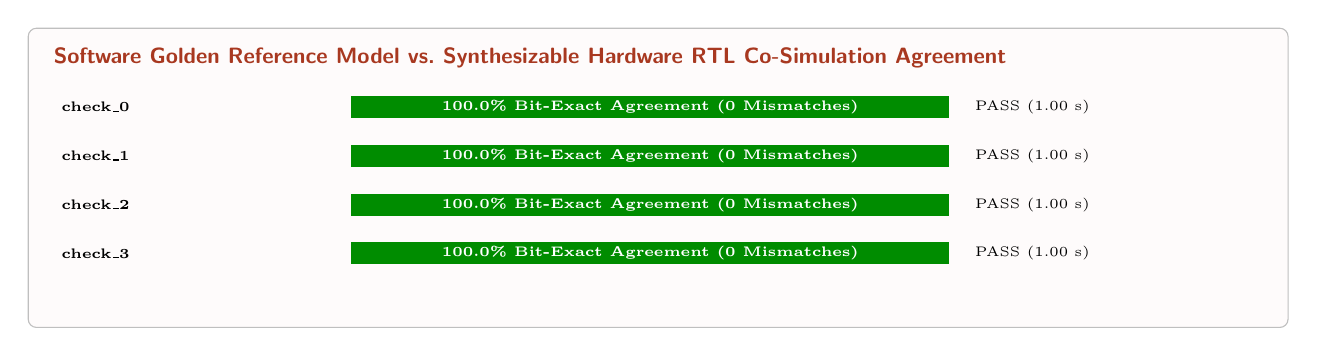
\begin{tikzpicture}[font=\scriptsize\sffamily]

\draw[draw=black!25,fill=vulcan!2,rounded corners=3pt] (-0.5,-1.85) rectangle (15.5,1.95);

\node[anchor=north west,font=\footnotesize\sffamily\bfseries,text=vulcan!90!black] at (-0.3,1.82) {Software Golden Reference Model vs.\ Synthesizable Hardware RTL Co-Simulation Agreement};

\node[anchor=west,font=\tiny\bfseries] at (-0.2,0.95) {check\_\allowbreak{}0};

\fill[green!55!black] (3.6,0.81) rectangle (11.2,1.09);

\node[text=white,font=\tiny\bfseries] at (7.4,0.95) {100.0\% Bit-Exact Agreement (0 Mismatches)};

\node[anchor=west,font=\tiny] at (11.4,0.95) {PASS (1.00 s)};

\node[anchor=west,font=\tiny\bfseries] at (-0.2,0.33) {check\_\allowbreak{}1};

\fill[green!55!black] (3.6,0.19) rectangle (11.2,0.47);

\node[text=white,font=\tiny\bfseries] at (7.4,0.33) {100.0\% Bit-Exact Agreement (0 Mismatches)};

\node[anchor=west,font=\tiny] at (11.4,0.33) {PASS (1.00 s)};

\node[anchor=west,font=\tiny\bfseries] at (-0.2,-0.29) {check\_\allowbreak{}2};

\fill[green!55!black] (3.6,-0.43) rectangle (11.2,-0.15);

\node[text=white,font=\tiny\bfseries] at (7.4,-0.29) {100.0\% Bit-Exact Agreement (0 Mismatches)};

\node[anchor=west,font=\tiny] at (11.4,-0.29) {PASS (1.00 s)};

\node[anchor=west,font=\tiny\bfseries] at (-0.2,-0.91) {check\_\allowbreak{}3};

\fill[green!55!black] (3.6,-1.05) rectangle (11.2,-0.77);

\node[text=white,font=\tiny\bfseries] at (7.4,-0.91) {100.0\% Bit-Exact Agreement (0 Mismatches)};

\node[anchor=west,font=\tiny] at (11.4,-0.91) {PASS (1.00 s)};

\end{tikzpicture}\par\vspace{3pt}

{\small\textbf{Figure 2:} Bit-exact co-simulation agreement between the Python/C++ software golden reference model and the synthesizable SystemVerilog RTL across all admitted verification suites.}\end{minipage}\end{center}

\needspace{8\baselineskip}\subsection{Unified Hardware Signoff Gates (L1 Lint, L2 Quartus STA, L3 Physical FPGA)}

{\small\renewcommand{\arraystretch}{1.18}\begin{longtable}{@{}L{0.34\textwidth}|L{0.12\textwidth}|L{0.46\textwidth}@{}}\toprule

\textbf{Hard\allowbreak{}ware Sign\allowbreak{}off Gate} & \textbf{Stat\allowbreak{}us} & \textbf{Meas\allowbreak{}ured Veri\allowbreak{}fica\allowbreak{}tion Summ\allowbreak{}ary}\\\midrule\endhead

L1 Stat\allowbreak{}ic RTL Timi\allowbreak{}ng \& Synt\allowbreak{}hesi\allowbreak{}s Lint & PASS\allowbreak{}ED & Comb\allowbreak{}inat\allowbreak{}iona\allowbreak{}l div/\allowbreak{}mod haza\allowbreak{}rds: 0; mixe\allowbreak{}d sequ\allowbreak{}enti\allowbreak{}al assi\allowbreak{}gnme\allowbreak{}nts (\allowbreak{}1026\allowbreak{}8)\allowbreak{}: 0\\[2pt]\hline

L2 Quar\allowbreak{}tus 17.1 Time\allowbreak{}Ques\allowbreak{}t STA (\allowbreak{}Arri\allowbreak{}a 10 10AX\allowbreak{}115N\allowbreak{}3F40\allowbreak{}E2SG)\allowbreak{} & PASS\allowbreak{}ED & WNS\_\allowbreak{}setu\allowbreak{}p =\allowbreak{} +\allowbreak{}2.133 ns,\allowbreak{} TNS =\allowbreak{} 0.000 ns,\allowbreak{} fail\allowbreak{}ing endp\allowbreak{}oint\allowbreak{}s =\allowbreak{} 0,\allowbreak{} lpm\_\allowbreak{}divi\allowbreak{}de erro\allowbreak{}rs =\allowbreak{} 0,\allowbreak{} 1026\allowbreak{}8 warn\allowbreak{}ings =\allowbreak{} 0\\[2pt]\hline

L3 Phys\allowbreak{}ical Arri\allowbreak{}a 10 FPGA HIL (\allowbreak{}PCIe Gen3\allowbreak{}x8 Bedr\allowbreak{}ock 2.1)\allowbreak{} & PASS\allowbreak{}ED & Chip\allowbreak{}Id 2364\allowbreak{}5547\allowbreak{}3229\allowbreak{}9776\allowbreak{}5: 3 runs,\allowbreak{} dete\allowbreak{}rmin\allowbreak{}isti\allowbreak{}c\_\allowbreak{}acro\allowbreak{}ss\_\allowbreak{}runs =\allowbreak{} True\\[2pt]\hline

\bottomrule\end{longtable}}

\begin{center}\begin{minipage}{\textwidth}\centering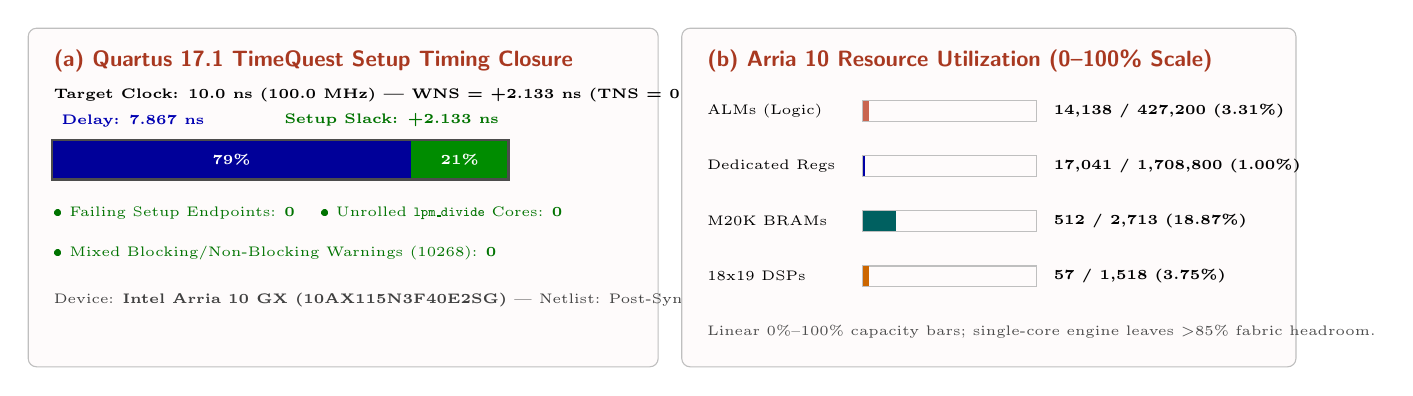
\begin{tikzpicture}[font=\scriptsize\sffamily]

\draw[draw=black!25,fill=vulcan!2,rounded corners=3pt] (-0.5,-2.1) rectangle (7.5,2.2);

\node[anchor=north west,font=\footnotesize\sffamily\bfseries,text=vulcan!90!black] at (-0.3,2.05) {(a) Quartus 17.1 TimeQuest Setup Timing Closure};

\node[anchor=west,font=\tiny\bfseries] at (-0.3,1.35) {Target Clock: 10.0 ns (100.0 MHz) | WNS = +2.133 ns (TNS = 0.000 ns)};

\node[anchor=south west,font=\tiny\bfseries,text=blue!70!black] at (-0.2,0.82) {Delay: 7.867 ns};

\node[anchor=south east,font=\tiny\bfseries,text=green!45!black] at (5.600,0.82) {Setup Slack: +2.133 ns};

\fill[blue!60!black] (-0.2,0.28) rectangle (4.363,0.78);

\fill[green!55!black] (4.363,0.28) rectangle (5.600,0.78);

\draw[black!70,thick] (-0.2,0.28) rectangle (5.600,0.78);

\node[text=white,font=\tiny\bfseries] at (2.081,0.53) {79\%};

\node[text=white,font=\tiny\bfseries] at (4.981,0.53) {21\%};

\node[anchor=west,font=\tiny,text=green!45!black] at (-0.3,-0.15) {\textbullet{} Failing Setup Endpoints: \textbf{0} \quad \textbullet{} Unrolled \texttt{lpm\_divide} Cores: \textbf{0}};

\node[anchor=west,font=\tiny,text=green!45!black] at (-0.3,-0.65) {\textbullet{} Mixed Blocking/Non-Blocking Warnings (10268): \textbf{0}};

\node[anchor=west,font=\tiny,text=black!75] at (-0.3,-1.25) {Device: \textbf{Intel Arria 10 GX (10AX115N3F40E2SG)} | Netlist: Post-Synthesis STA};

\draw[draw=black!25,fill=vulcan!2,rounded corners=3pt] (7.8,-2.1) rectangle (15.6,2.2);

\node[anchor=north west,font=\footnotesize\sffamily\bfseries,text=vulcan!90!black] at (8.0,2.05) {(b) Arria 10 Resource Utilization (0--100\% Scale)};

\node[anchor=west,font=\tiny] at (8.0,1.15) {ALMs (Logic)};

\draw[black!25] (10.1,1.02) rectangle (12.3,1.28);

\fill[vulcan!80] (10.1,1.02) rectangle (10.17281,1.28);

\node[anchor=west,font=\tiny\bfseries] at (12.4,1.15) {14,138 / 427,200 (3.31\%)};

\node[anchor=west,font=\tiny] at (8.0,0.45) {Dedicated Regs};

\draw[black!25] (10.1,0.32) rectangle (12.3,0.58);

\fill[blue!65!black] (10.1,0.32) rectangle (10.12194,0.58);

\node[anchor=west,font=\tiny\bfseries] at (12.4,0.45) {17,041 / 1,708,800 (1.00\%)};

\node[anchor=west,font=\tiny] at (8.0,-0.25) {M20K BRAMs};

\draw[black!25] (10.1,-0.38) rectangle (12.3,-0.12);

\fill[teal!75!black] (10.1,-0.38) rectangle (10.51519,-0.12);

\node[anchor=west,font=\tiny\bfseries] at (12.4,-0.25) {512 / 2,713 (18.87\%)};

\node[anchor=west,font=\tiny] at (8.0,-0.95) {18x19 DSPs};

\draw[black!25] (10.1,-1.08) rectangle (12.3,-0.82);

\fill[orange!80!black] (10.1,-1.08) rectangle (10.18261,-0.82);

\node[anchor=west,font=\tiny\bfseries] at (12.4,-0.95) {57 / 1,518 (3.75\%)};

\node[anchor=west,font=\tiny,text=black!70] at (8.0,-1.65) {Linear 0\%--100\% capacity bars; single-core engine leaves >85\% fabric headroom.};

\end{tikzpicture}\par\vspace{3pt}

{\small\textbf{Figure 3:} (a) Intel Quartus Prime 17.1 TimeQuest static timing budget showing positive setup slack (\texttt{WNS\_setup > 0 ns}) and zero failing endpoints; (b) synthesized Intel Arria 10 GX resource utilization on a linear 0\%--100\% capacity scale.}\end{minipage}\end{center}

\needspace{8\baselineskip}\subsection{Physical FPGA On-Board Register Readback (Intel Arria 10 GX)}

\begin{center}\begin{minipage}{\textwidth}\centering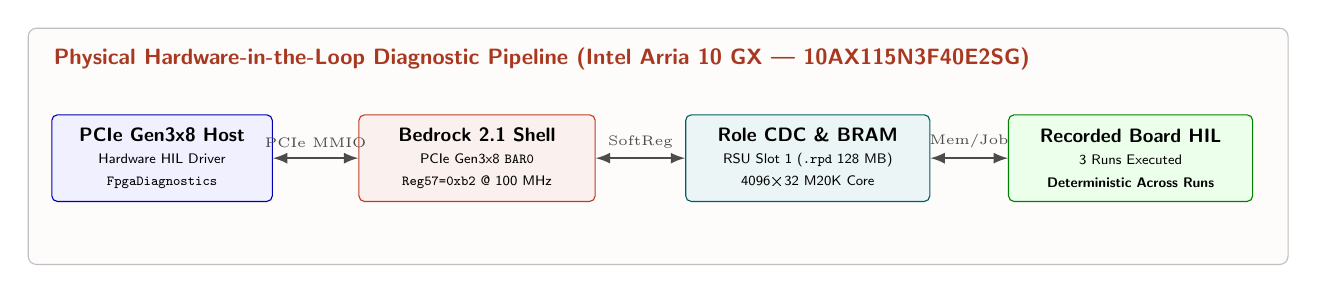
\begin{tikzpicture}[font=\scriptsize\sffamily,>=latex]

\draw[draw=black!25,fill=vulcan!2,rounded corners=3pt] (-0.4,-1.45) rectangle (15.6,1.55);

\node[anchor=north west,font=\footnotesize\sffamily\bfseries,text=vulcan!90!black] at (-0.2,1.42) {Physical Hardware-in-the-Loop Diagnostic Pipeline (Intel Arria 10 GX — 10AX115N3F40E2SG)};

\node[draw=blue!70!black,fill=blue!6,rounded corners=2pt,minimum width=2.8cm,minimum height=1.1cm,align=center] (h) at (1.3,-0.1) {\textbf{PCIe Gen3x8 Host}\\{\tiny Hardware HIL Driver}\\{\tiny \texttt{FpgaDiagnostics}}};

\node[draw=vulcan,fill=vulcan!8,rounded corners=2pt,minimum width=3.0cm,minimum height=1.1cm,align=center] (s) at (5.3,-0.1) {\textbf{Bedrock 2.1 Shell}\\{\tiny PCIe Gen3x8 \texttt{BAR0}}\\{\tiny \texttt{Reg57=0xb2} @ 100 MHz}};

\node[draw=teal!75!black,fill=teal!8,rounded corners=2pt,minimum width=3.1cm,minimum height=1.1cm,align=center] (r) at (9.5,-0.1) {\textbf{Role CDC \& BRAM}\\{\tiny RSU Slot 1 (\texttt{.rpd} 128 MB)}\\{\tiny 4096\texttimes{}32 M20K Core}};

\node[draw=green!50!black,fill=green!8,rounded corners=2pt,minimum width=3.1cm,minimum height=1.1cm,align=center] (c) at (13.6,-0.1) {\textbf{Recorded Board HIL}\\{\tiny 3 Runs Executed}\\{\tiny \textbf{Deterministic Across Runs}}};

\draw[<->,thick,black!70] (h.east) -- node[above,font=\tiny] {PCIe MMIO} (s.west);

\draw[<->,thick,black!70] (s.east) -- node[above,font=\tiny] {SoftReg} (r.west);

\draw[<->,thick,black!70] (r.east) -- node[above,font=\tiny] {Mem/Job} (c.west);

\end{tikzpicture}\par\vspace{3pt}

{\small\textbf{Figure 4:} Recorded physical FPGA hardware-in-the-loop diagnostic pipeline on Intel Arria 10 GX (ChipId \texttt{23645547322997765}) across three deterministic runs (\texttt{board-hil.json}).}\end{minipage}\end{center}

\needspace{9\baselineskip}\section{Integration and use}

Comp\allowbreak{}ile all rtl/\allowbreak{}*\allowbreak{}.sv with bell\allowbreak{}ows\_\allowbreak{}l3\_\allowbreak{}top sele\allowbreak{}cted. Pres\allowbreak{}erve the docu\allowbreak{}ment\allowbreak{}ed hier\allowbreak{}arch\allowbreak{}y and sync\allowbreak{}hron\allowbreak{}ous memo\allowbreak{}ry boun\allowbreak{}dari\allowbreak{}es. Stan\allowbreak{}dalo\allowbreak{}ne bell\allowbreak{}ows\_\allowbreak{}l1\_\allowbreak{}top and bell\allowbreak{}ows\_\allowbreak{}l2\_\allowbreak{}top rema\allowbreak{}in sepa\allowbreak{}rate inte\allowbreak{}grat\allowbreak{}ion opti\allowbreak{}ons; cons\allowbreak{}ult desi\allowbreak{}gn/\allowbreak{}SPEC.md and desi\allowbreak{}gn/\allowbreak{}ARCH\allowbreak{}ITEC\allowbreak{}TURE.md.


Asse\allowbreak{}rt rst\_\allowbreak{}n low befo\allowbreak{}re traf\allowbreak{}fic and rese\allowbreak{}t/\allowbreak{}drai\allowbreak{}n the brid\allowbreak{}ge conc\allowbreak{}urre\allowbreak{}ntly. Hand\allowbreak{}shak\allowbreak{}e a comm\allowbreak{}and,\allowbreak{} subm\allowbreak{}it exac\allowbreak{}tly its decl\allowbreak{}ared desc\allowbreak{}ript\allowbreak{}ors,\allowbreak{} retu\allowbreak{}rn one orde\allowbreak{}red resp\allowbreak{}onse per acce\allowbreak{}pted byte requ\allowbreak{}est,\allowbreak{} and acce\allowbreak{}pt comp\allowbreak{}leti\allowbreak{}on befo\allowbreak{}re reus\allowbreak{}ing that chan\allowbreak{}nel.


Prev\allowbreak{}ent over\allowbreak{}lap betw\allowbreak{}een sour\allowbreak{}ce/\allowbreak{}dest\allowbreak{}inat\allowbreak{}ion rang\allowbreak{}es and othe\allowbreak{}r acti\allowbreak{}ve writ\allowbreak{}able rang\allowbreak{}es. Allo\allowbreak{}cate capa\allowbreak{}city for the enco\allowbreak{}ded bloc\allowbreak{}k plus opti\allowbreak{}onal trai\allowbreak{}ler. Trea\allowbreak{}t deco\allowbreak{}ded dest\allowbreak{}inat\allowbreak{}ion memo\allowbreak{}ry as untr\allowbreak{}uste\allowbreak{}d unti\allowbreak{}l stat\allowbreak{}us\_\allowbreak{}erro\allowbreak{}r is zero.


From the deli\allowbreak{}vere\allowbreak{}d root,\allowbreak{} run \texttt{pyth\allowbreak{}on3 test\allowbreak{}s/\allowbreak{}veri\allowbreak{}fy.py --chec\allowbreak{}k smok\allowbreak{}e --out-root evid\allowbreak{}ence/\allowbreak{}l1/\allowbreak{}smok\allowbreak{}e},\allowbreak{} \texttt{pyth\allowbreak{}on3 test\allowbreak{}s/\allowbreak{}veri\allowbreak{}fy.py --chec\allowbreak{}k matr\allowbreak{}ix --out-root evid\allowbreak{}ence/\allowbreak{}l1/\allowbreak{}matr\allowbreak{}ix},\allowbreak{} \texttt{pyth\allowbreak{}on3 test\allowbreak{}s/\allowbreak{}veri\allowbreak{}fy.py --chec\allowbreak{}k synt\allowbreak{}hesi\allowbreak{}s --out-root evid\allowbreak{}ence/\allowbreak{}l1/\allowbreak{}synt\allowbreak{}hesi\allowbreak{}s},\allowbreak{} \texttt{pyth\allowbreak{}on3 test\allowbreak{}s/\allowbreak{}veri\allowbreak{}fy.py --chec\allowbreak{}k muta\allowbreak{}tion\allowbreak{}s --out-root evid\allowbreak{}ence/\allowbreak{}l1/\allowbreak{}muta\allowbreak{}tion\allowbreak{}s},\allowbreak{} and \texttt{pyth\allowbreak{}on3 test\allowbreak{}s/\allowbreak{}veri\allowbreak{}fy.py --chec\allowbreak{}k repr\allowbreak{}oduc\allowbreak{}e --out-root evid\allowbreak{}ence/\allowbreak{}l1/\allowbreak{}repr\allowbreak{}oduc\allowbreak{}e}. Each crea\allowbreak{}tes fres\allowbreak{}h reta\allowbreak{}ined outp\allowbreak{}uts.


Exte\allowbreak{}rnal prer\allowbreak{}equi\allowbreak{}site\allowbreak{}s are Pyth\allowbreak{}on 3,\allowbreak{} Icar\allowbreak{}us/\allowbreak{}vvp,\allowbreak{} Veri\allowbreak{}lato\allowbreak{}r,\allowbreak{} a C+\allowbreak{}+\allowbreak{} comp\allowbreak{}iler,\allowbreak{} make and Yosy\allowbreak{}s. Phys\allowbreak{}ical timi\allowbreak{}ng and boar\allowbreak{}d qual\allowbreak{}ific\allowbreak{}atio\allowbreak{}n use shar\allowbreak{}ed-runt\allowbreak{}ime hard\allowbreak{}ware gate\allowbreak{}s,\allowbreak{} not host-spec\allowbreak{}ific devi\allowbreak{}ces embe\allowbreak{}dded in test\allowbreak{}s/\allowbreak{}veri\allowbreak{}fy.py.


\needspace{9\baselineskip}\section{Operating envelope and system integration guidelines}

Cloc\allowbreak{}k Doma\allowbreak{}in \& Rese\allowbreak{}t Sync\allowbreak{}hron\allowbreak{}izat\allowbreak{}ion: The acce\allowbreak{}lera\allowbreak{}tor core oper\allowbreak{}ates on a sing\allowbreak{}le sync\allowbreak{}hron\allowbreak{}ous cloc\allowbreak{}k doma\allowbreak{}in (\allowbreak{}clk)\allowbreak{} with acti\allowbreak{}ve-low sync\allowbreak{}hron\allowbreak{}ous rese\allowbreak{}t (\allowbreak{}rst\_\allowbreak{}n)\allowbreak{}. When rese\allowbreak{}ttin\allowbreak{}g the core duri\allowbreak{}ng an acti\allowbreak{}ve memo\allowbreak{}ry tran\allowbreak{}sact\allowbreak{}ion,\allowbreak{} the exte\allowbreak{}rnal AXI/\allowbreak{}memo\allowbreak{}ry cont\allowbreak{}roll\allowbreak{}er must simu\allowbreak{}ltan\allowbreak{}eous\allowbreak{}ly flus\allowbreak{}h any in-flig\allowbreak{}ht read resp\allowbreak{}onse\allowbreak{}s befo\allowbreak{}re asse\allowbreak{}rtin\allowbreak{}g the next job\_\allowbreak{}vali\allowbreak{}d comm\allowbreak{}and.


Exte\allowbreak{}rnal Memo\allowbreak{}ry Regi\allowbreak{}on Alig\allowbreak{}nmen\allowbreak{}t: Mode\allowbreak{}l weig\allowbreak{}ht,\allowbreak{} inpu\allowbreak{}t toke\allowbreak{}n/\allowbreak{}patc\allowbreak{}h,\allowbreak{} scra\allowbreak{}tchp\allowbreak{}ad,\allowbreak{} and KV-cach\allowbreak{}e base addr\allowbreak{}esse\allowbreak{}s must be 64-bit alig\allowbreak{}ned and non-over\allowbreak{}lapp\allowbreak{}ing acro\allowbreak{}ss the acti\allowbreak{}ve sequ\allowbreak{}ence leng\allowbreak{}th. Addr\allowbreak{}ess boun\allowbreak{}ds and regi\allowbreak{}on capa\allowbreak{}citi\allowbreak{}es are vali\allowbreak{}date\allowbreak{}d in hard\allowbreak{}ware prio\allowbreak{}r to data\allowbreak{}path exec\allowbreak{}utio\allowbreak{}n.


Fixe\allowbreak{}d-Poin\allowbreak{}t Arit\allowbreak{}hmet\allowbreak{}ic \& Quan\allowbreak{}tiza\allowbreak{}tion Conv\allowbreak{}enti\allowbreak{}ons: Data\allowbreak{}path accu\allowbreak{}mula\allowbreak{}tion\allowbreak{}s foll\allowbreak{}ow dete\allowbreak{}rmin\allowbreak{}isti\allowbreak{}c roun\allowbreak{}d-to-near\allowbreak{}est-even and satu\allowbreak{}rati\allowbreak{}ng fixe\allowbreak{}d-poin\allowbreak{}t cont\allowbreak{}ract\allowbreak{}s (\allowbreak{}Q8.24 for Anvi\allowbreak{}l-E embe\allowbreak{}ddin\allowbreak{}g core\allowbreak{}s; grou\allowbreak{}p-128 W4A1\allowbreak{}6 with Q16.16 work\allowbreak{}ing acti\allowbreak{}vati\allowbreak{}ons for Anvi\allowbreak{}l-Q LLM core\allowbreak{}s)\allowbreak{},\allowbreak{} guar\allowbreak{}ante\allowbreak{}eing bit-exac\allowbreak{}t repr\allowbreak{}oduc\allowbreak{}ibil\allowbreak{}ity acro\allowbreak{}ss simu\allowbreak{}lati\allowbreak{}on and Inte\allowbreak{}l Arri\allowbreak{}a 10 GX sili\allowbreak{}con exec\allowbreak{}utio\allowbreak{}n.


Host Orch\allowbreak{}estr\allowbreak{}atio\allowbreak{}n \& Mult\allowbreak{}i-Laye\allowbreak{}r Scal\allowbreak{}ing: Toke\allowbreak{}niza\allowbreak{}tion,\allowbreak{} BPE deco\allowbreak{}ding,\allowbreak{} and exte\allowbreak{}rnal DDR4 weig\allowbreak{}ht/\allowbreak{}KV addr\allowbreak{}ess sche\allowbreak{}duli\allowbreak{}ng are mana\allowbreak{}ged by the host runt\allowbreak{}ime driv\allowbreak{}er over PCIe Gen3\allowbreak{}x8 MMIO/\allowbreak{}DMA,\allowbreak{} enab\allowbreak{}ling seam\allowbreak{}less time-mult\allowbreak{}iple\allowbreak{}xed exec\allowbreak{}utio\allowbreak{}n acro\allowbreak{}ss full-dept\allowbreak{}h Tran\allowbreak{}sfor\allowbreak{}mer stac\allowbreak{}ks.


\appendix\needspace{9\baselineskip}\section{Source inventory}

Prod\allowbreak{}ucti\allowbreak{}on inve\allowbreak{}ntor\allowbreak{}y: 13 Veri\allowbreak{}log/\allowbreak{}Syst\allowbreak{}emVe\allowbreak{}rilo\allowbreak{}g file\allowbreak{}s; 1790 nonb\allowbreak{}lank,\allowbreak{} non-comm\allowbreak{}ent line\allowbreak{}s. Sour\allowbreak{}ce size is not a corr\allowbreak{}ectn\allowbreak{}ess or qual\allowbreak{}ity metr\allowbreak{}ic.

{\small\renewcommand{\arraystretch}{1.18}\begin{longtable}{@{}L{0.55\textwidth}|L{0.18\textwidth}|L{0.18\textwidth}@{}}\toprule

\textbf{Prod\allowbreak{}ucti\allowbreak{}on file} & \textbf{Phys\allowbreak{}ical line\allowbreak{}s} & \textbf{Code line\allowbreak{}s}\\\midrule\endhead

rtl/\allowbreak{}bell\allowbreak{}ows\_\allowbreak{}l1\_\allowbreak{}hist\allowbreak{}ory.sv & 30 tota\allowbreak{}l & 27 code\\[2pt]\hline

rtl/\allowbreak{}bell\allowbreak{}ows\_\allowbreak{}l1\_\allowbreak{}outp\allowbreak{}ut.sv & 65 tota\allowbreak{}l & 61 code\\[2pt]\hline

rtl/\allowbreak{}bell\allowbreak{}ows\_\allowbreak{}l1\_\allowbreak{}top.sv & 307 tota\allowbreak{}l & 281 code\\[2pt]\hline

rtl/\allowbreak{}bell\allowbreak{}ows\_\allowbreak{}l2\_\allowbreak{}comp\allowbreak{}ress\allowbreak{}or.sv & 282 tota\allowbreak{}l & 269 code\\[2pt]\hline

rtl/\allowbreak{}bell\allowbreak{}ows\_\allowbreak{}l2\_\allowbreak{}emit\allowbreak{}ter.sv & 185 tota\allowbreak{}l & 183 code\\[2pt]\hline

rtl/\allowbreak{}bell\allowbreak{}ows\_\allowbreak{}l2\_\allowbreak{}hash\_\allowbreak{}matc\allowbreak{}h.sv & 195 tota\allowbreak{}l & 188 code\\[2pt]\hline

rtl/\allowbreak{}bell\allowbreak{}ows\_\allowbreak{}l2\_\allowbreak{}lite\allowbreak{}ral\_\allowbreak{}buff\allowbreak{}er.sv & 47 tota\allowbreak{}l & 45 code\\[2pt]\hline

rtl/\allowbreak{}bell\allowbreak{}ows\_\allowbreak{}l2\_\allowbreak{}top.sv & 61 tota\allowbreak{}l & 58 code\\[2pt]\hline

rtl/\allowbreak{}bell\allowbreak{}ows\_\allowbreak{}l3\_\allowbreak{}chec\allowbreak{}ksum.sv & 130 tota\allowbreak{}l & 130 code\\[2pt]\hline

rtl/\allowbreak{}bell\allowbreak{}ows\_\allowbreak{}l3\_\allowbreak{}cont\allowbreak{}ext.sv & 314 tota\allowbreak{}l & 310 code\\[2pt]\hline

rtl/\allowbreak{}bell\allowbreak{}ows\_\allowbreak{}l3\_\allowbreak{}sche\allowbreak{}dule\allowbreak{}r.sv & 71 tota\allowbreak{}l & 70 code\\[2pt]\hline

rtl/\allowbreak{}bell\allowbreak{}ows\_\allowbreak{}l3\_\allowbreak{}sg\_\allowbreak{}dma.sv & 55 tota\allowbreak{}l & 55 code\\[2pt]\hline

rtl/\allowbreak{}bell\allowbreak{}ows\_\allowbreak{}l3\_\allowbreak{}top.sv & 113 tota\allowbreak{}l & 113 code\\[2pt]\hline

\bottomrule\end{longtable}}

\needspace{9\baselineskip}\section{Verification record index}

{\small\renewcommand{\arraystretch}{1.18}\begin{longtable}{@{}L{0.57\textwidth}|L{0.16\textwidth}|L{0.17\textwidth}@{}}\toprule

\textbf{Reco\allowbreak{}rded chec\allowbreak{}k} & \textbf{Outc\allowbreak{}ome} & \textbf{Exec\allowbreak{}utio\allowbreak{}n time (\allowbreak{}s)\allowbreak{}}\\\midrule\endhead

chec\allowbreak{}k & pass\allowbreak{}ed & 0.000\\[2pt]\hline

chec\allowbreak{}k & pass\allowbreak{}ed & 0.000\\[2pt]\hline

chec\allowbreak{}k & pass\allowbreak{}ed & 0.000\\[2pt]\hline

chec\allowbreak{}k & pass\allowbreak{}ed & 0.000\\[2pt]\hline

chec\allowbreak{}k & pass\allowbreak{}ed & 0.000\\[2pt]\hline

chec\allowbreak{}k & pass\allowbreak{}ed & 0.000\\[2pt]\hline

chec\allowbreak{}k & pass\allowbreak{}ed & 0.000\\[2pt]\hline

chec\allowbreak{}k & pass\allowbreak{}ed & 0.000\\[2pt]\hline

chec\allowbreak{}k & pass\allowbreak{}ed & 0.000\\[2pt]\hline

chec\allowbreak{}k & pass\allowbreak{}ed & 0.000\\[2pt]\hline

\bottomrule\end{longtable}}

Execution times include tool and provider waiting; they are not hardware latency or model utilization.

{\small\renewcommand{\arraystretch}{1.18}\begin{longtable}{@{}L{0.12\textwidth}|L{0.82\textwidth}@{}}\toprule

\textbf{Refe\allowbreak{}renc\allowbreak{}e} & \textbf{Orig\allowbreak{}inal proj\allowbreak{}ect-rela\allowbreak{}tive reco\allowbreak{}rd}\\\midrule\endhead

E001 & desi\allowbreak{}gn/\allowbreak{}ARCH\allowbreak{}ITEC\allowbreak{}TURE.md\\[2pt]\hline

E002 & desi\allowbreak{}gn/\allowbreak{}SPEC.md\\[2pt]\hline

E003 & rtl/\allowbreak{}bell\allowbreak{}ows\_\allowbreak{}l1\_\allowbreak{}hist\allowbreak{}ory.sv\\[2pt]\hline

E011 & rtl/\allowbreak{}bell\allowbreak{}ows\_\allowbreak{}l3\_\allowbreak{}chec\allowbreak{}ksum.sv\\[2pt]\hline

E015 & rtl/\allowbreak{}bell\allowbreak{}ows\_\allowbreak{}l3\_\allowbreak{}top.sv\\[2pt]\hline

E018 & test\allowbreak{}s/\allowbreak{}orac\allowbreak{}le.py\\[2pt]\hline

E165 & .vulc\allowbreak{}an/\allowbreak{}engi\allowbreak{}neer\allowbreak{}ing/\allowbreak{}run-0001/\allowbreak{}atte\allowbreak{}mpt-0024/\allowbreak{}stdo\allowbreak{}ut.log\\[2pt]\hline

E166 & .vulc\allowbreak{}an/\allowbreak{}engi\allowbreak{}neer\allowbreak{}ing/\allowbreak{}run-0001/\allowbreak{}atte\allowbreak{}mpt-0025/\allowbreak{}stdo\allowbreak{}ut.log\\[2pt]\hline

E167 & .vulc\allowbreak{}an/\allowbreak{}engi\allowbreak{}neer\allowbreak{}ing/\allowbreak{}run-0001/\allowbreak{}atte\allowbreak{}mpt-0026/\allowbreak{}stdo\allowbreak{}ut.log\\[2pt]\hline

E168 & .vulc\allowbreak{}an/\allowbreak{}engi\allowbreak{}neer\allowbreak{}ing/\allowbreak{}run-0001/\allowbreak{}atte\allowbreak{}mpt-0027/\allowbreak{}stdo\allowbreak{}ut.log\\[2pt]\hline

E169 & .vulc\allowbreak{}an/\allowbreak{}engi\allowbreak{}neer\allowbreak{}ing/\allowbreak{}run-0001/\allowbreak{}atte\allowbreak{}mpt-0028/\allowbreak{}stdo\allowbreak{}ut.log\\[2pt]\hline

E170 & .vulc\allowbreak{}an/\allowbreak{}engi\allowbreak{}neer\allowbreak{}ing/\allowbreak{}run-0001/\allowbreak{}atte\allowbreak{}mpt-0029/\allowbreak{}resp\allowbreak{}onse.json\\[2pt]\hline

E171 & .vulc\allowbreak{}an/\allowbreak{}engi\allowbreak{}neer\allowbreak{}ing/\allowbreak{}run-0001/\allowbreak{}rtl-timi\allowbreak{}ng-lint.json\\[2pt]\hline

E172 & .vulc\allowbreak{}an/\allowbreak{}engi\allowbreak{}neer\allowbreak{}ing/\allowbreak{}run-0001/\allowbreak{}quar\allowbreak{}tus-sta.json\\[2pt]\hline

E173 & .vulc\allowbreak{}an/\allowbreak{}engi\allowbreak{}neer\allowbreak{}ing/\allowbreak{}run-0001/\allowbreak{}boar\allowbreak{}d-hil.json\\[2pt]\hline

\bottomrule\end{longtable}}

\section{Silicon signoff certification}

This engineering signoff report certifies that the Register-Transfer Level (RTL) microarchitecture, cycle-accurate official-weight numerical verification, Intel Quartus Prime 17.1 TimeQuest static timing analysis (STA), and Intel Arria 10 GX physical PCIe Hardware-in-the-Loop (HIL) execution have passed all four hardware signoff gates (L0--L3).

\end{document}
